The overall design of this project can be split into three phases:

\begin{enumerate}
    \item Pre-training: in this phase, I train two equivariant GNN models on the RES task, using the ATOM 3D dataset \cite{atom-3d} (Section \ref{phase1-res-task}).
    \item Mutation generation: in this phase, I repurpose the models trained in Phase 1 to generate possible amino acid mutations for a subset of proteins from the ProteinGym dataset \cite{tranception} (Section \ref{sec:mutation-generation}); I then evaluate how much better these mutations are than the wildtype\footnote{The wildtype is the non-mutated protein.} in Chapter \ref{results}.
    \item Protein fitness prediction: in the last phase, I use the models trained in Phase 1 to generate position scores for every possible amino acid in a sequence. I use these scores as features in a ridge regression model in order to predict the fitness of each single-point mutation in the ProteinGym dataset \cite{tranception} (Section \ref{protein-fitness-prediction}).
\end{enumerate}

\section{Pre-training: residue identity prediction}
\label{phase1-res-task}

I use the ATOM3D dataset \cite{atom-3d}, comprising of atomic environments extracted from non-redundant structures in the Protein Data Bank (PDB). This dataset serves as the foundation for formulating the RES task as a classification problem. The rest of this section will outline the details of the dataset used (Section \ref{res-dataset}), an overview of the training pipeline (Section \ref{training-overview}), and the two equivariant models trained on the RES task (Sections \ref{the-gvp-math} and Sections \ref{eqgat-math}). 

\subsection{Dataset details}
\label{res-dataset}
The dataset contains a number of high-resolution molecules from the PDB. 
For each molecule, the creators provide samples of local atomic environments. 
Each local environment is composed of all atoms within a 10 \AA ~radius of the $\text{C}_{\beta}$ atom of the masked amino acid.
The sample contains the indices of the atoms to remove from the original PDB file, as well as the target amino acid.
We use these samples to generate masked local environments to feed into the ML model. These environments are atom graphs; edges are drawn between any two nodes that are \textbf{less that 4.5\AA ~apart}. Figure \ref{protein_pipeline} illustrates this pipeline. 

\begin{figure}
    \centering
    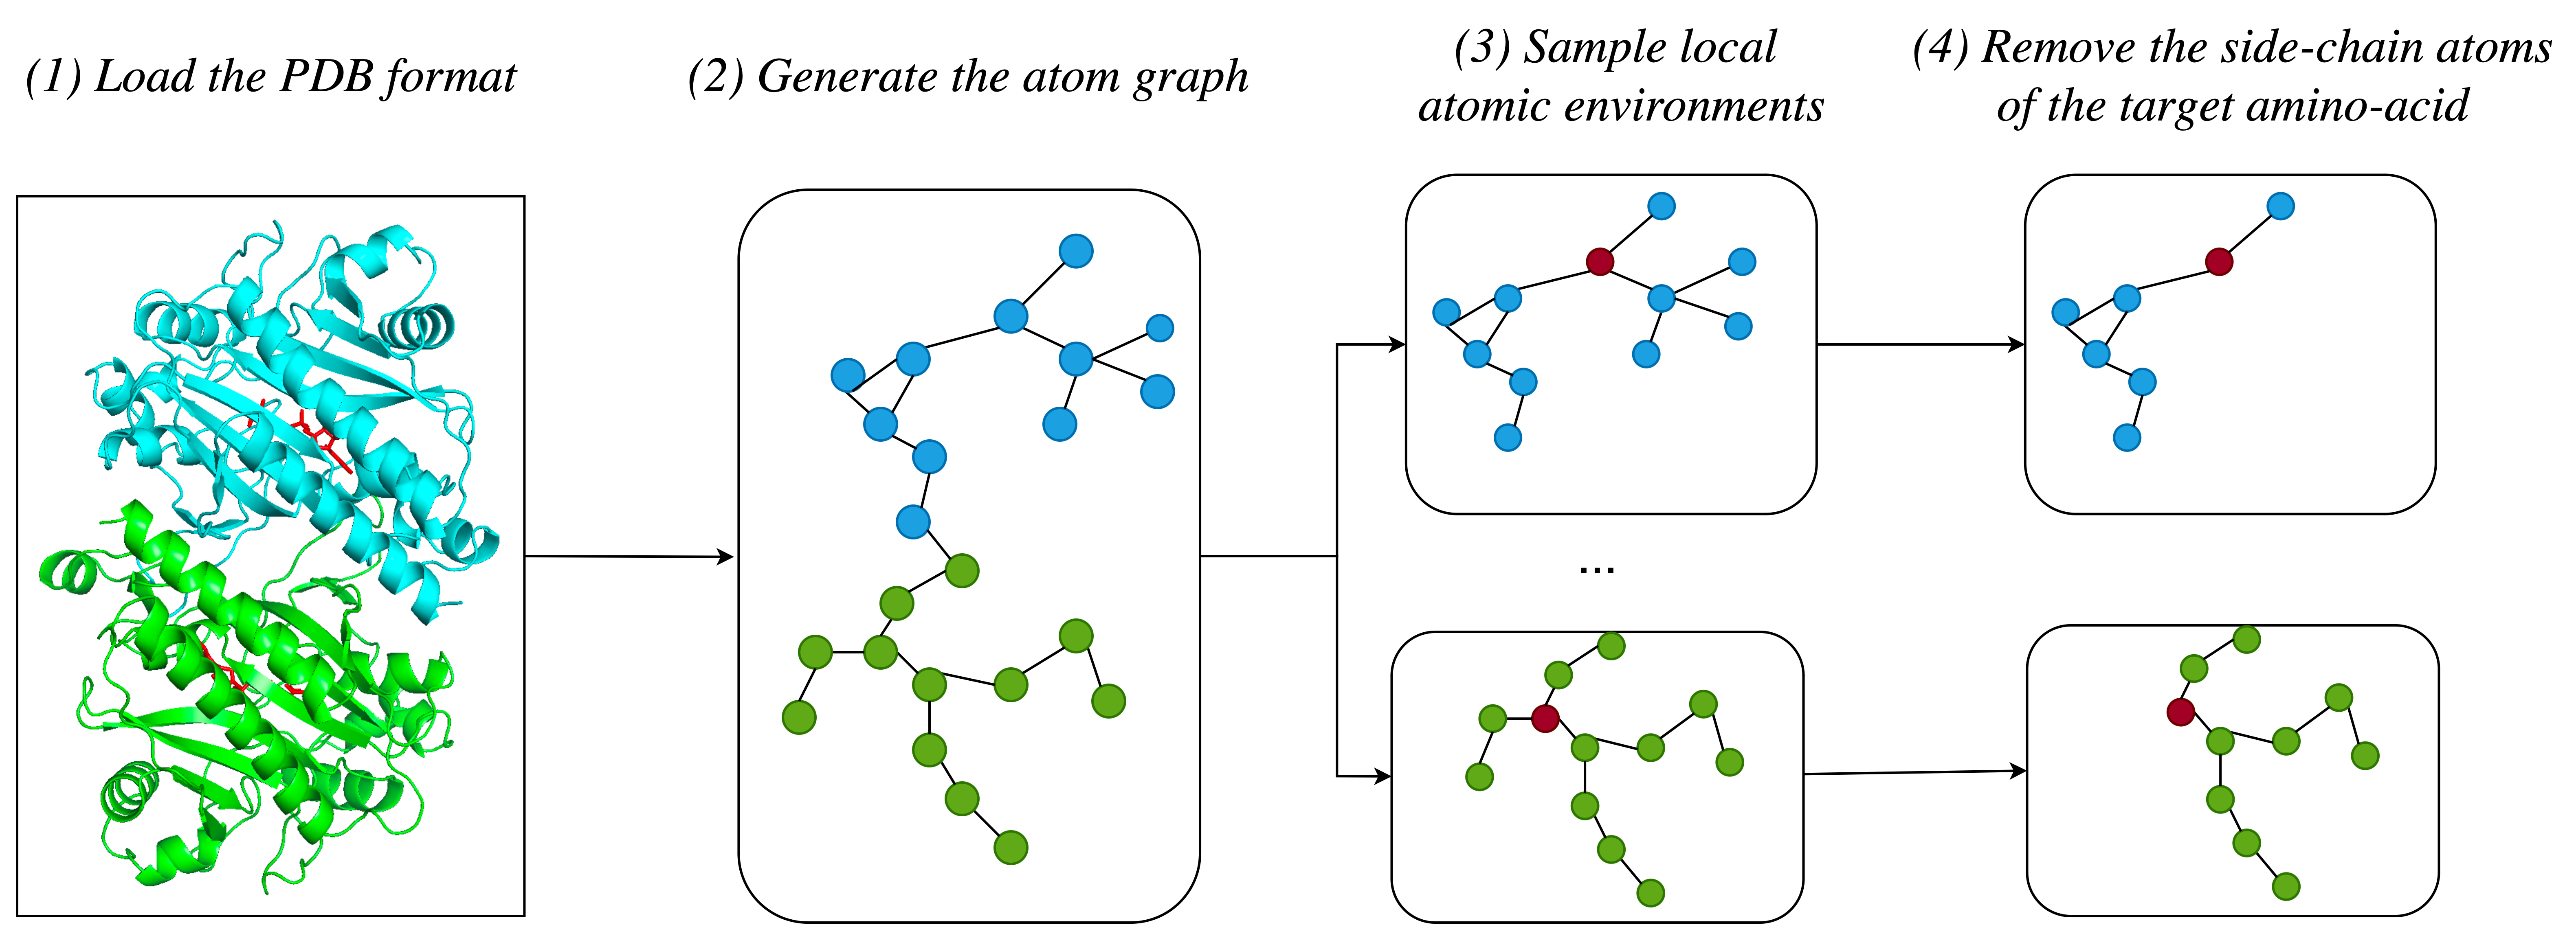
\includegraphics[width=\textwidth]{masters-report/figures/graph-pipeline.png}
    \caption{Data generation pipeline for the RES task. The local atomic environments are sampled according to indices provided by the ATOM3D dataset \cite{atom-3d}. The red nodes represent the $\text{C}_{\alpha}$ carbons of their respective amino acid residues; these are the nodes we are interested in classifying correctly.}
    \label{protein_pipeline}
\end{figure}

\paragraph{Side-chain masking.} As mentioned in Section \ref{amino-acids}, all amino acid residues share the same underlying \textit{backbone} structure. Due to this reason, when masking the target amino acid, the authors of the RES dataset only remove its \textit{side-chain} atoms. The side-chain is always bound to the $\text{C}_{\alpha}$ atom of the residue (as explained in Section \ref{amino-acids}), so we train the ML model to classify this atom as one of the 20 naturally occurring amino acids.


\paragraph{Dataset splitting and class imbalances.}
Many molecules have common ancestors, and CATH topology classes \cite{Dawson2017CATH} were introduced in order to group these protein domains into superfamilies when there is sufficient evidence they have diverged from a common ancestor. The creators of the ATOM3D RES dataset split the train, validation and test datasets such that proteins belonging to topology classes that appear in the training set will not appear in the test set. This is done as a way to properly assess the generalisation performance of the models, since otherwise the models can memorise the general attributes of a certain CATH class. 

Moreover, not all amino acids appear with the same frequency in real-life molecules. To deal with possible class imbalances, the authors downsample the local environments of the training set to the frequency of the least common amino acid (cysteine). Table \ref{dataset_stats} provides a summary of the statistics of the full RES ATOM3D dataset.


\begin{table}[]
    \centering
    \begin{tabular}{@{}lccc@{}}
    \toprule
    Dataset    & No. molecules & Avg no. samples/molecule & Avg no. atoms/sample \\ \midrule
    Train      & 21072           & 181                       & 622                   \\
    Validation & 962             & 199                       & 612                   \\
    Test       & 3303            & 196                       & 613                   \\ \bottomrule
    \end{tabular}
    \caption{Statistics of the ATOM3D RES dataset.}
    \label{dataset_stats}
\end{table}

\subsection{Training overview}
\label{training-overview}
The training pipeline is summarised in Figure \ref{res-task}. We treat this task as a node classification task, and train the model to predict the most likely side-chain for a target $\text{C}_{\alpha}$ atom given its local environment.

\begin{figure}[!h]
    \centering
    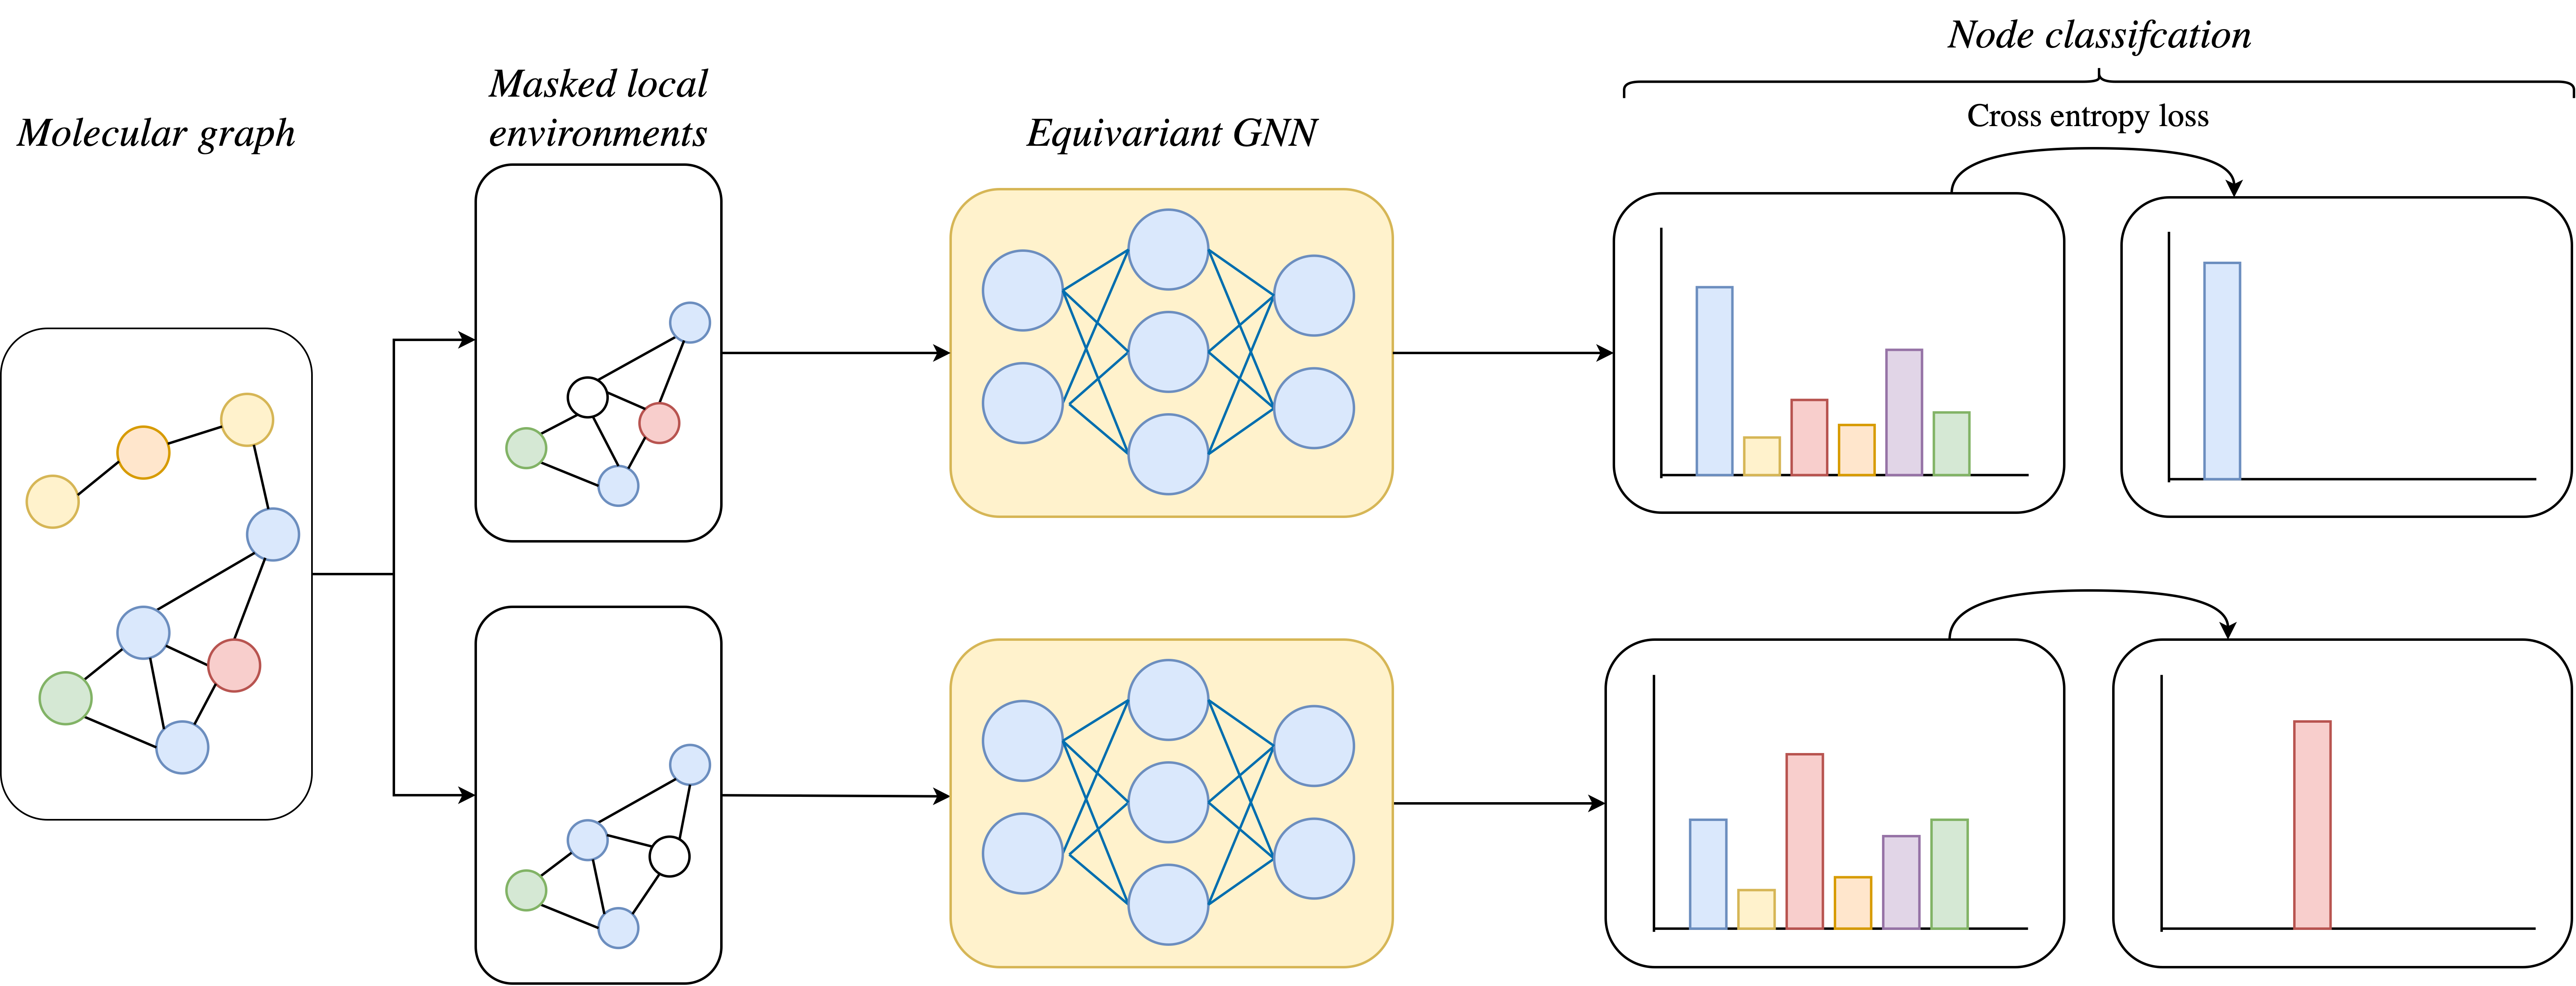
\includegraphics[width=\textwidth]{masters-report/figures/training-pipeline.png}
    \caption{Diagram of phase 1, illustrating the pipeline used in training the models on the RES task.}
    \label{res-task}
\end{figure}
\paragraph{Graph readout.} More formally, for a given graph $\mathcal{G} = (\mathcal{V}, \mathcal{E})$ with nodes $i,j \in \mathcal{V}$ and edges $(i \rightarrow j) \in \mathcal{E}$ for which we have initial scalar and vector node features $\mathbf{H}\in\mathbb{R}^{|\mathcal{V}|\times n}\times\mathbb{R}^{|\mathcal{V}|\times 3 \times \nu}$, as well as scalar and vector edge features $\mathbf{E}\in\mathbb{R}^{|\mathcal{E}|\times m}\times\mathbb{R}^{|\mathcal{E}|\times 3 \times \eta}$, we first consider a \textit{masked} version of this graph, $\mathcal{G}_t=(\mathcal{V}_t, \mathcal{E}_t)$, from which we have removed all the atoms of the side-chain attached to the node $t$ (representing an $\text{C}_{\alpha}$ atom). 

We then formally define the GNN model $\mathbf{G}_{\theta_1}:\mathbb{R}^{|\mathcal{V}_t|\times n}\times\mathbb{R}^{|\mathcal{V}_t|\times 3 \times \nu}\times\mathbb{R}^{|\mathcal{E}_t|\times m}\times\mathbb{R}^{|\mathcal{E}_t|\times 3 \times \eta}\rightarrow \mathbb{R}^{|\mathcal{V}_t|\times o}$ that takes as input the node and edge features and returns final node features  $\mathbf{H}_{\text{out}}$:
\begin{equation}
    \mathbf{H}_{\text{out}} = \mathbf{G}_{\theta_1}(\mathbf{H}_t, \mathbf{E}_t)
\end{equation}
where $\mathbf{H}_t$ and $\mathbf{E}_t$ represent the node and edge features for all nodes and edges that exist in the masked graph $\mathcal{G}_t$.

Since we are interested in predicting the type of amino acid corresponding to the masked side-chain of node $t$, we define a pooling function $\text{pool}:\mathbb{N}\times\mathbb{R}^{|\mathcal{V}_t|\times o}\rightarrow \mathbb{R}^o$ that retrieves the final features of node $t$:
\begin{equation}
    \text{pool}(t, \mathbf{H}_{\text{out}}) = [\mathbf{H}_{\text{out}}]_t
\end{equation}

We pass $\mathbf{h}_{t} = \text{pool}(t, \mathbf{H}_{\text{out}})$ through a multi-layer perceptron $\text{MLP}_{\theta_2}:\mathbb{R}^o\rightarrow \mathbb{R}^{20}$ to obtain the final scores associated to each of the 20 naturally occuring amino acids:
\begin{equation}
    l = \text{MLP}_{\theta_2}(\mathbf{h}_t)
\label{logit-scores}
\end{equation}
Hence, the masking process, the overall GNN model, and the downstream MLP form the node classification function $f_{\gamma}^t:\mathbb{R}^{|\mathcal{V}|\times n}\times\mathbb{R}^{|\mathcal{V}|\times 3 \times \nu}\times\mathbb{R}^{|\mathcal{E}|\times m}\times\mathbb{R}^{|\mathcal{E}|\times 3 \times \eta}\rightarrow \mathbb{R}^{20}$ with learnable parameters $\gamma = \{\theta_1, \theta_2\}$:
\begin{equation}
    f_{\gamma}^t(\mathbf{H}, \mathbf{E}) = \text{MLP}_{\theta_2}(\text{pool}(t, \mathbf{G}_{\theta_1}(\mathbf{H}_t, \mathbf{E}_t)))
\label{full-formalism}
\end{equation}

The \textbf{loss function} of our model quantifies the dissimilarity between the predicted probability distribution associated with scores $l$ obtained in Equation \ref{logit-scores} and the true probability distribution associated with the target class, also known in the literature as the cross-entropy loss:
\begin{equation}
    \mathcal{L}(l, y) = -\log\frac{\exp({l_y})}{\sum_{c=1}^{20} \exp({l_c})}
\label{logits}
\end{equation}
where $y \in \{1,2,\dots,20\}$ is the true class of target node $t$.
\subsection{The geometric vector perceptron}
\label{the-gvp-math}
The first of the two architectures employed for pre-training in this project is the Geometric Vector Perceptron (GVP). The GVP is an equivariant learning module introduced by \citet{gvp1}. It lays the foundation for the GVP-GNN model, an equivariant GNN that has proven to be a successful architecture for many structure-based molecular tasks \cite{gvp1, gvp2}. In this work, we are using the second version of the GVP-GNN architecture, as described in \citet{gvp2}. 

\paragraph{The GVP module.}
The GVP module can learn both scalar-valued and vector-valued functions over geometric vectors and scalars; it can be thought of as generalising the concept of a Multi-Layer Perceptron to vectors, hence its ability to learn geometric properties of molecules. 

Borrowing some notation from \citet{gvp1}, for each node in a graph we can define the tuple $\mathbf{h} = (\mathbf{s}, \mathbf{V})$ of scalar features $\mathbf{s}\in\mathbb{R}^{n}$ and vector features $\mathbf{V}\in \mathbb{R}^{\nu\times 3}$. Then, the GVP computes updated features $\mathbf{h}'=(\mathbf{s}', \mathbf{V}') \in \mathbb{R}^m\times\mathbb{R}^{\mu \times 3}$ as can be seen in Algorithm \ref{gvp-algo}.
\begin{figure}[!h]
    \begin{minipage}[b]{0.3\textwidth}
    \centering
    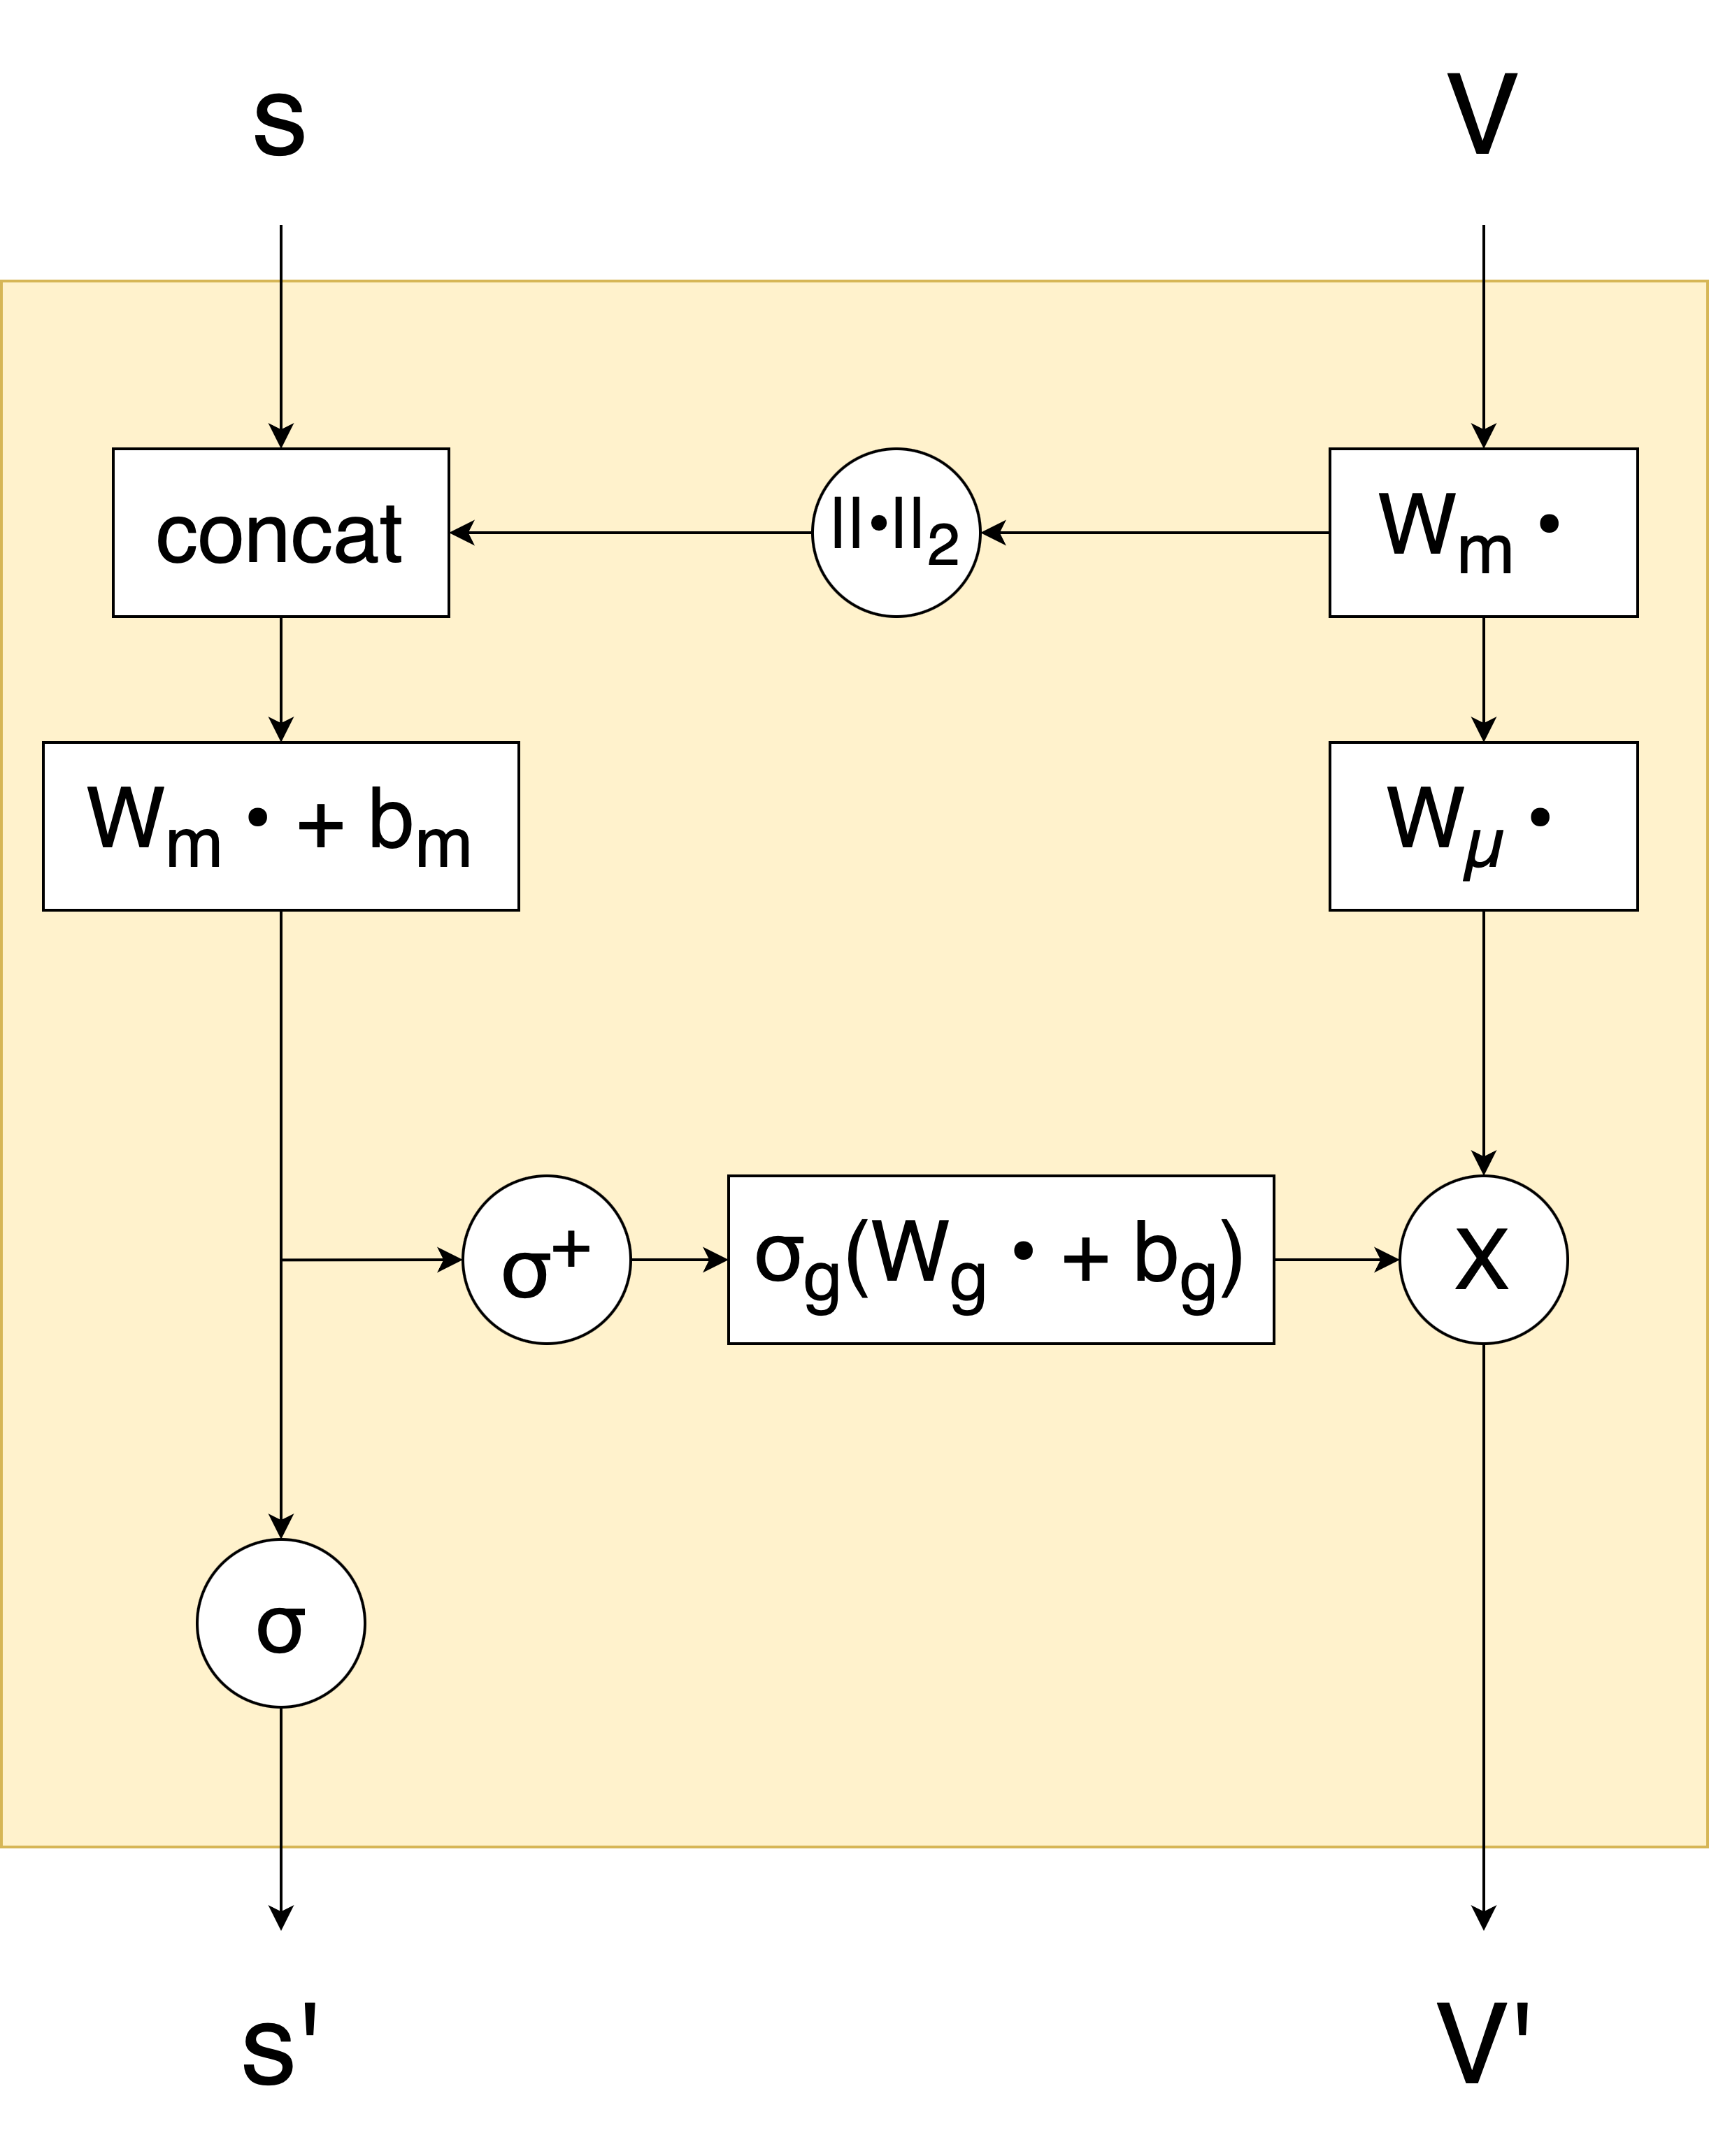
\includegraphics[width=\textwidth]{masters-report/figures/gvp.png}
    \label{fig:image}
  \end{minipage}
  \hfill
  \begin{minipage}[b]{0.65\textwidth}
    % \begin{algorithm}
% \caption{Geometric Vector Perceptron}
\hline
\begin{algorithmic}
\renewcommand{\algorithmicrequire}{\textbf{Input:}}
\renewcommand{\algorithmicensure}{\textbf{Output:}}
\Require{Scalar and vector feats. $(\mathbf{s}, \mathbf{V}) \in \mathbb{R}^n\times \mathbb{R}^{\nu \times 3}$}
\Ensure{Scalar and vector feats. $(\mathbf{s}', \mathbf{V}')\in \mathbb{R}^n\times\mathbb{R}^{\mu\times 3}$}
\State $h \gets \max(\nu, \mu)$

\State $V_h \gets \mathbf{W}_h\mathbf{V} \in \mathbb{R}^{h\times3}$

\State $V_{\mu} \gets \mathbf{W}_{\mu}\mathbf{V}_h \in \mathbb{R}^{\mu\times 3}$

\State $\mathbf{s}_h\gets ||V_h||_2$ (row-wise) $\in \mathbb{R}^h$

\State $\mathbf{v}_{\mu} \gets ||V_{\mu}||_2$ (row-wise) $\in \mathbb{R}^{\mu}$

\State $\mathbf{s}_{h + n} \gets \text{concat}(\mathbf{s}_h, \mathbf{s})\in\mathbb{R}^{h + n}$

\State $\mathbf{s}_m \gets \mathbf{W}_m\mathbf{s}_{h+n}+\mathbf{b}\in \mathbb{R}^m$

\State $\mathbf{s}' \gets \sigma(\mathbf{s}_m)\in \mathbb{R}^m $

\State $\mathbf{V}' \gets \sigma_g(\mathbf{W}_g[\sigma^{+}(\mathbf{s}_m)] + \mathbf{b}_g) \circledcirc \mathbf{V}_{\mu}$ (row-wise) $\in \mathbb{R}^{\mu \times 3}$
\\
\Return $(\mathbf{s}', \mathbf{V}')$
\end{algorithmic}
\hline
% \end{algorithm}

  \end{minipage}
\caption{\textit{(Left)} An illustration of the data flow of the module; \textit{(Right)} Algorithm showing the computation involved in a GVP module.  Both the pseudocode and the illustration are adapted from \cite{gvp2}.}
\label{gvp-algo}
\end{figure}

\paragraph{The message-passing framework.} The GVP module can be incorporated in the message-passing framework to create a \textit{GVP convolutional layer}. If $\mathbf{h}_{\mathcal{V}}^{(j)}$ are the node features of node $j$ and $\mathbf{h}_{\mathcal{E}}^{(j\rightarrow i)}$ are the edge features of edge $(j \rightarrow i)$, then the module creates the message $\mathbf{m}^{(j\rightarrow i)}$ passed from node $j$ to node $i$ as follows:
\begin{equation}
\mathbf{m}^{(j\rightarrow i)} = g_1\Big(\text{concat}(\mathbf{h}_{\mathcal{V}}^{(j)}, ~~\mathbf{h}_{\mathcal{E}}^{(j \rightarrow i)})\Big) 
\end{equation}
Assuming $k$ is the number of incoming messages, we aggregate them according to:
\begin{equation}
\mathbf{m}_{\mathcal{V}}^{(i)}= \text{LayerNorm}\Big(\mathbf{h}_{\mathcal{V}}^{(i)} + \frac{1}{k}\text{Dropout}\big(\sum_{(j \rightarrow i)\in\mathcal{E}}\mathbf{m}^{(j\rightarrow i)}\big)\Big)
\label{aggregation}
\end{equation}
We follow this with a \textit{feed-forward point-wise} layer to update the node embeddings:
\begin{equation}
    \mathbf{h}_{\mathcal{V}}^{(i)}= \text{LayerNorm}\Big(\mathbf{m}_{\mathcal{V}}^{(i)} + \text{Dropout}\big(g_2(\mathbf{m}_{\mathcal{V}}^{(i)})\big)\Big)
\label{update}
\end{equation}
Functions $g_1$ and $g_2$ are compositions of three and two GVP modules, respectively.

\paragraph{Layer normalisation and dropout.} Dropout \cite{dropout} is a regularisation technique that randomly ``drops out'' a portion of the neurons during training, while layer normalisation \cite{layernorm} is a technique that normalises the activations of neurons within a layer to address the problem of internal covariate shift. Both techniques are widely used in practice to avoid overfitting. 

When dealing with scalar features, the equations \ref{aggregation} and \ref{update} use the standard implementations of these two layers. However, when dealing with vector features, \citet{gvp1} modify the Dropout layer to ``drop'' entire 3D vectors. Additionally, they define layer normalisation for vector features to scale the row vectors of $\mathbf{V} =[\mathbf{v}_1, \dots, \mathbf{v}_{\nu}]$, where $\nu$ is the number of vector features per node, such that the root-mean-square norm is equal to 1: 
\begin{equation}
    \mathbf{V} \leftarrow \mathbf{V}/\sqrt{\frac{1}{\nu}||\mathbf{V}||_2^2} ~~\in \mathbb{R}^{\nu\times 3}  
\end{equation}


The final architecture is composed of GVP modules, layer normalisation modules and GVP convolutional layers, as illustrated in Figure \ref{gvp-architecture}.
\begin{figure}
    \centering
    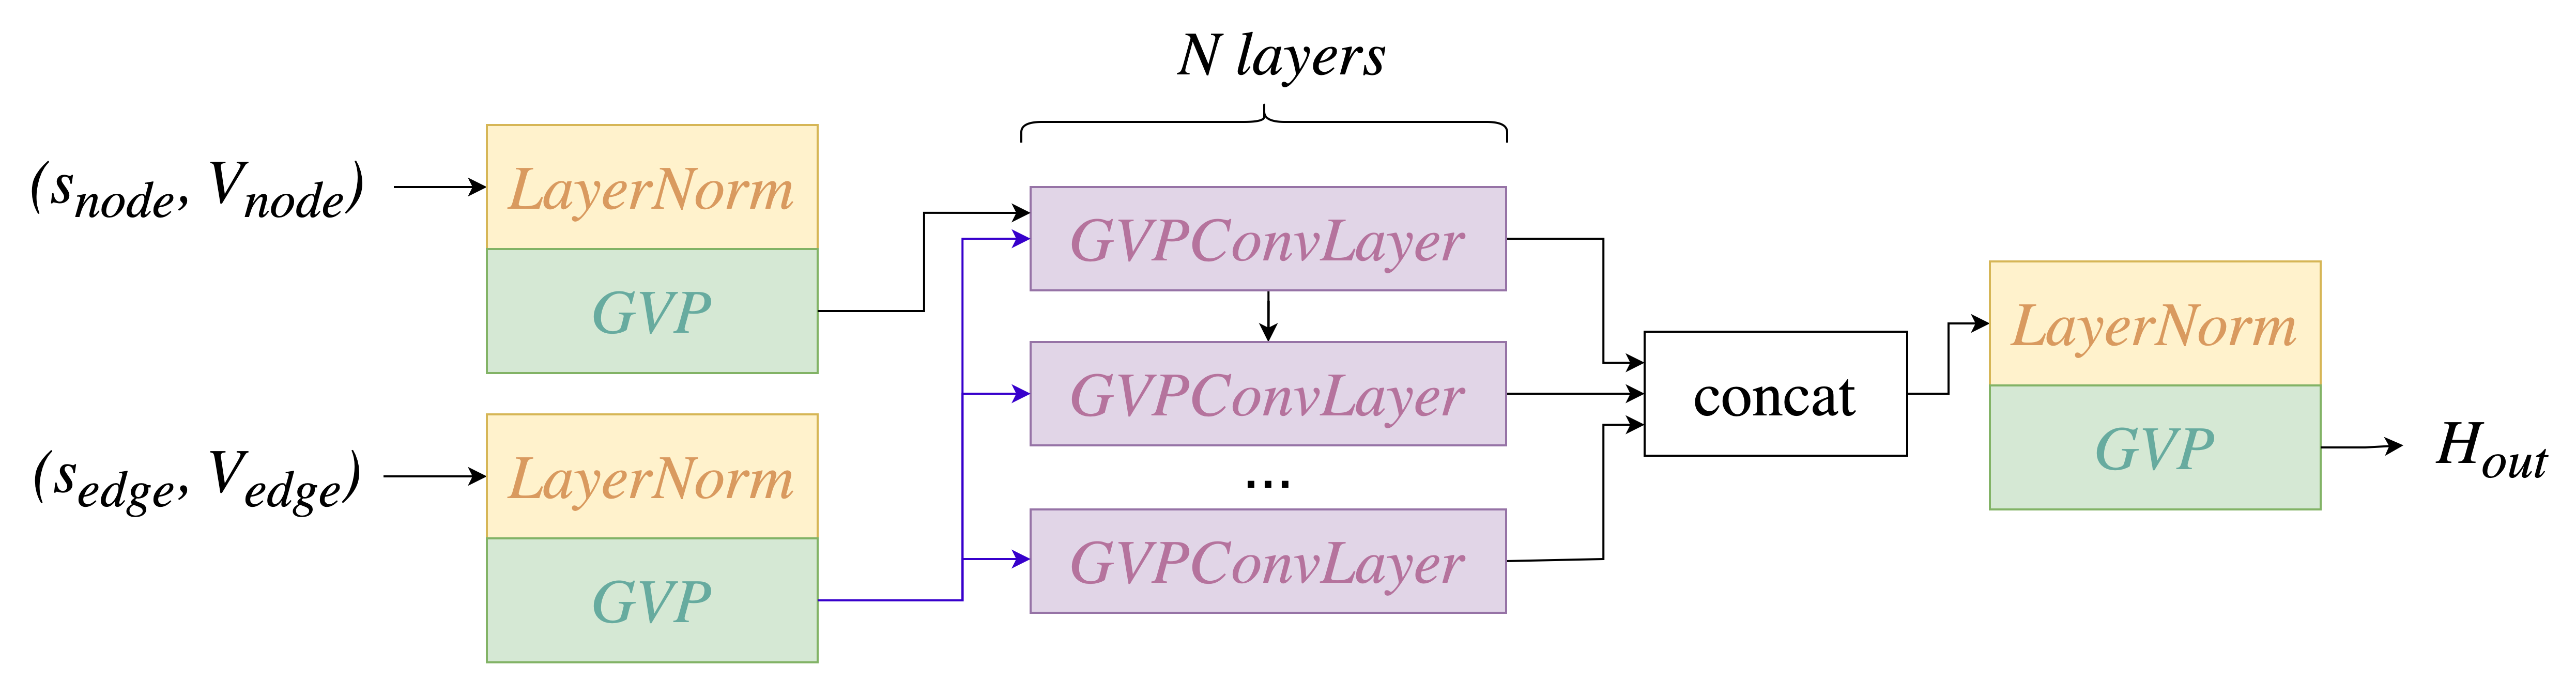
\includegraphics[width=\textwidth]{masters-report/figures/gvp-architecture.png}
    \caption{Overall architecture of the GVP-GNN model.}
    \label{gvp-architecture}
\end{figure}

\paragraph{Initial features.} 
The initial features used on the GVP-GNN architecture are separated into node features $(\mathbf{s}_{\text{node}}, \mathbf{V}_{\text{node}})$ and edge features $(\mathbf{s}_{\text{edge}}, \mathbf{V}_{\text{edge}})$. We obtain the scalar node features by passing its node type $z_{\text{node}}$ through a trainable embedding layer to obtain $\mathbf{s}_{\text{node}} = \text{embed}(z_{\text{node}})$, where $\text{embed}:\mathcal{A}\rightarrow \mathbb{R}^n$. All of the initial node vector features $\mathbf{V}_{\text{node}}$ are set to $\vec{\mathbf{0}}$.

To obtain the scalar edge features $\mathbf{s}_{\text{edge}}$, for each edge from node $i$ to node $j$ we encode the interatomic distance $d_{ji}$ in terms of Gaussian radial basis functions (RBFs). The reason for encoding the distance using RBFs is that these functions are non-zero only within a specified radius. This property enables them to capture local interactions between atoms while minimising the influence of distant nodes. Using these encodings instead of the plain Euclidean distance allows the model to learn how to treat different length scales in separate manners.

More formally, for hyperparameter $\epsilon\in\mathbb{R}_{+}$ controlling the smoothness of the basis function, we define the encoding of $d_{ji}$ to be:
\begin{equation}
    \text{GBF}_{\epsilon}(d_{ji}) = e^{-(\epsilon d_{ji})^2}
\end{equation}
I use 16 different $\epsilon$ values, evenly spaced between 0 to 20, rendering the final scalar edge features $\mathbf{s}_{ij} \in \mathbb{R}^{16}$. For the vector edge embeddings I compute the normalised edge direction: $\vec{\mathbf{v}}_{ij} = \frac{\mathbf{p}_i - \mathbf{p}_j}{||\mathbf{p}_i - \mathbf{p}_j||_2}$. 

\subsection{The equivariant graph attention network}
\label{eqgat-math}
The second EGNN architecture used in this project is the equivariant graph attention network introduced by \citet{eqgat}. A brief introduction into self-attention mechanisms is presented before diving into the specifics of this EGNN model.

Attention in neural networks refers to a mechanism that enables the network to focus on specific parts of the input data or relevant information while processing a task. It is inspired by human attention and aims to improve the network's ability to handle long sequences or complex patterns. The most popular attention mechanism to date was introduced by \citet{vaswani2017attention} and lies at the core of the Transformer architecture. 

The attention mechanism typically involves two components: a \textbf{query} and a set of \textbf{key-value pairs}. The query represents the information the network is currently processing, while the key-value pairs represent the contextual information or memory. The attention mechanism computes the similarity between the query and the keys to obtain \textit{attention weights}, which determine the importance of each value. Figure \ref{attention} illustrates the conceptual pipeline of a self-attention module.

\begin{figure}[!h]
    \centering
    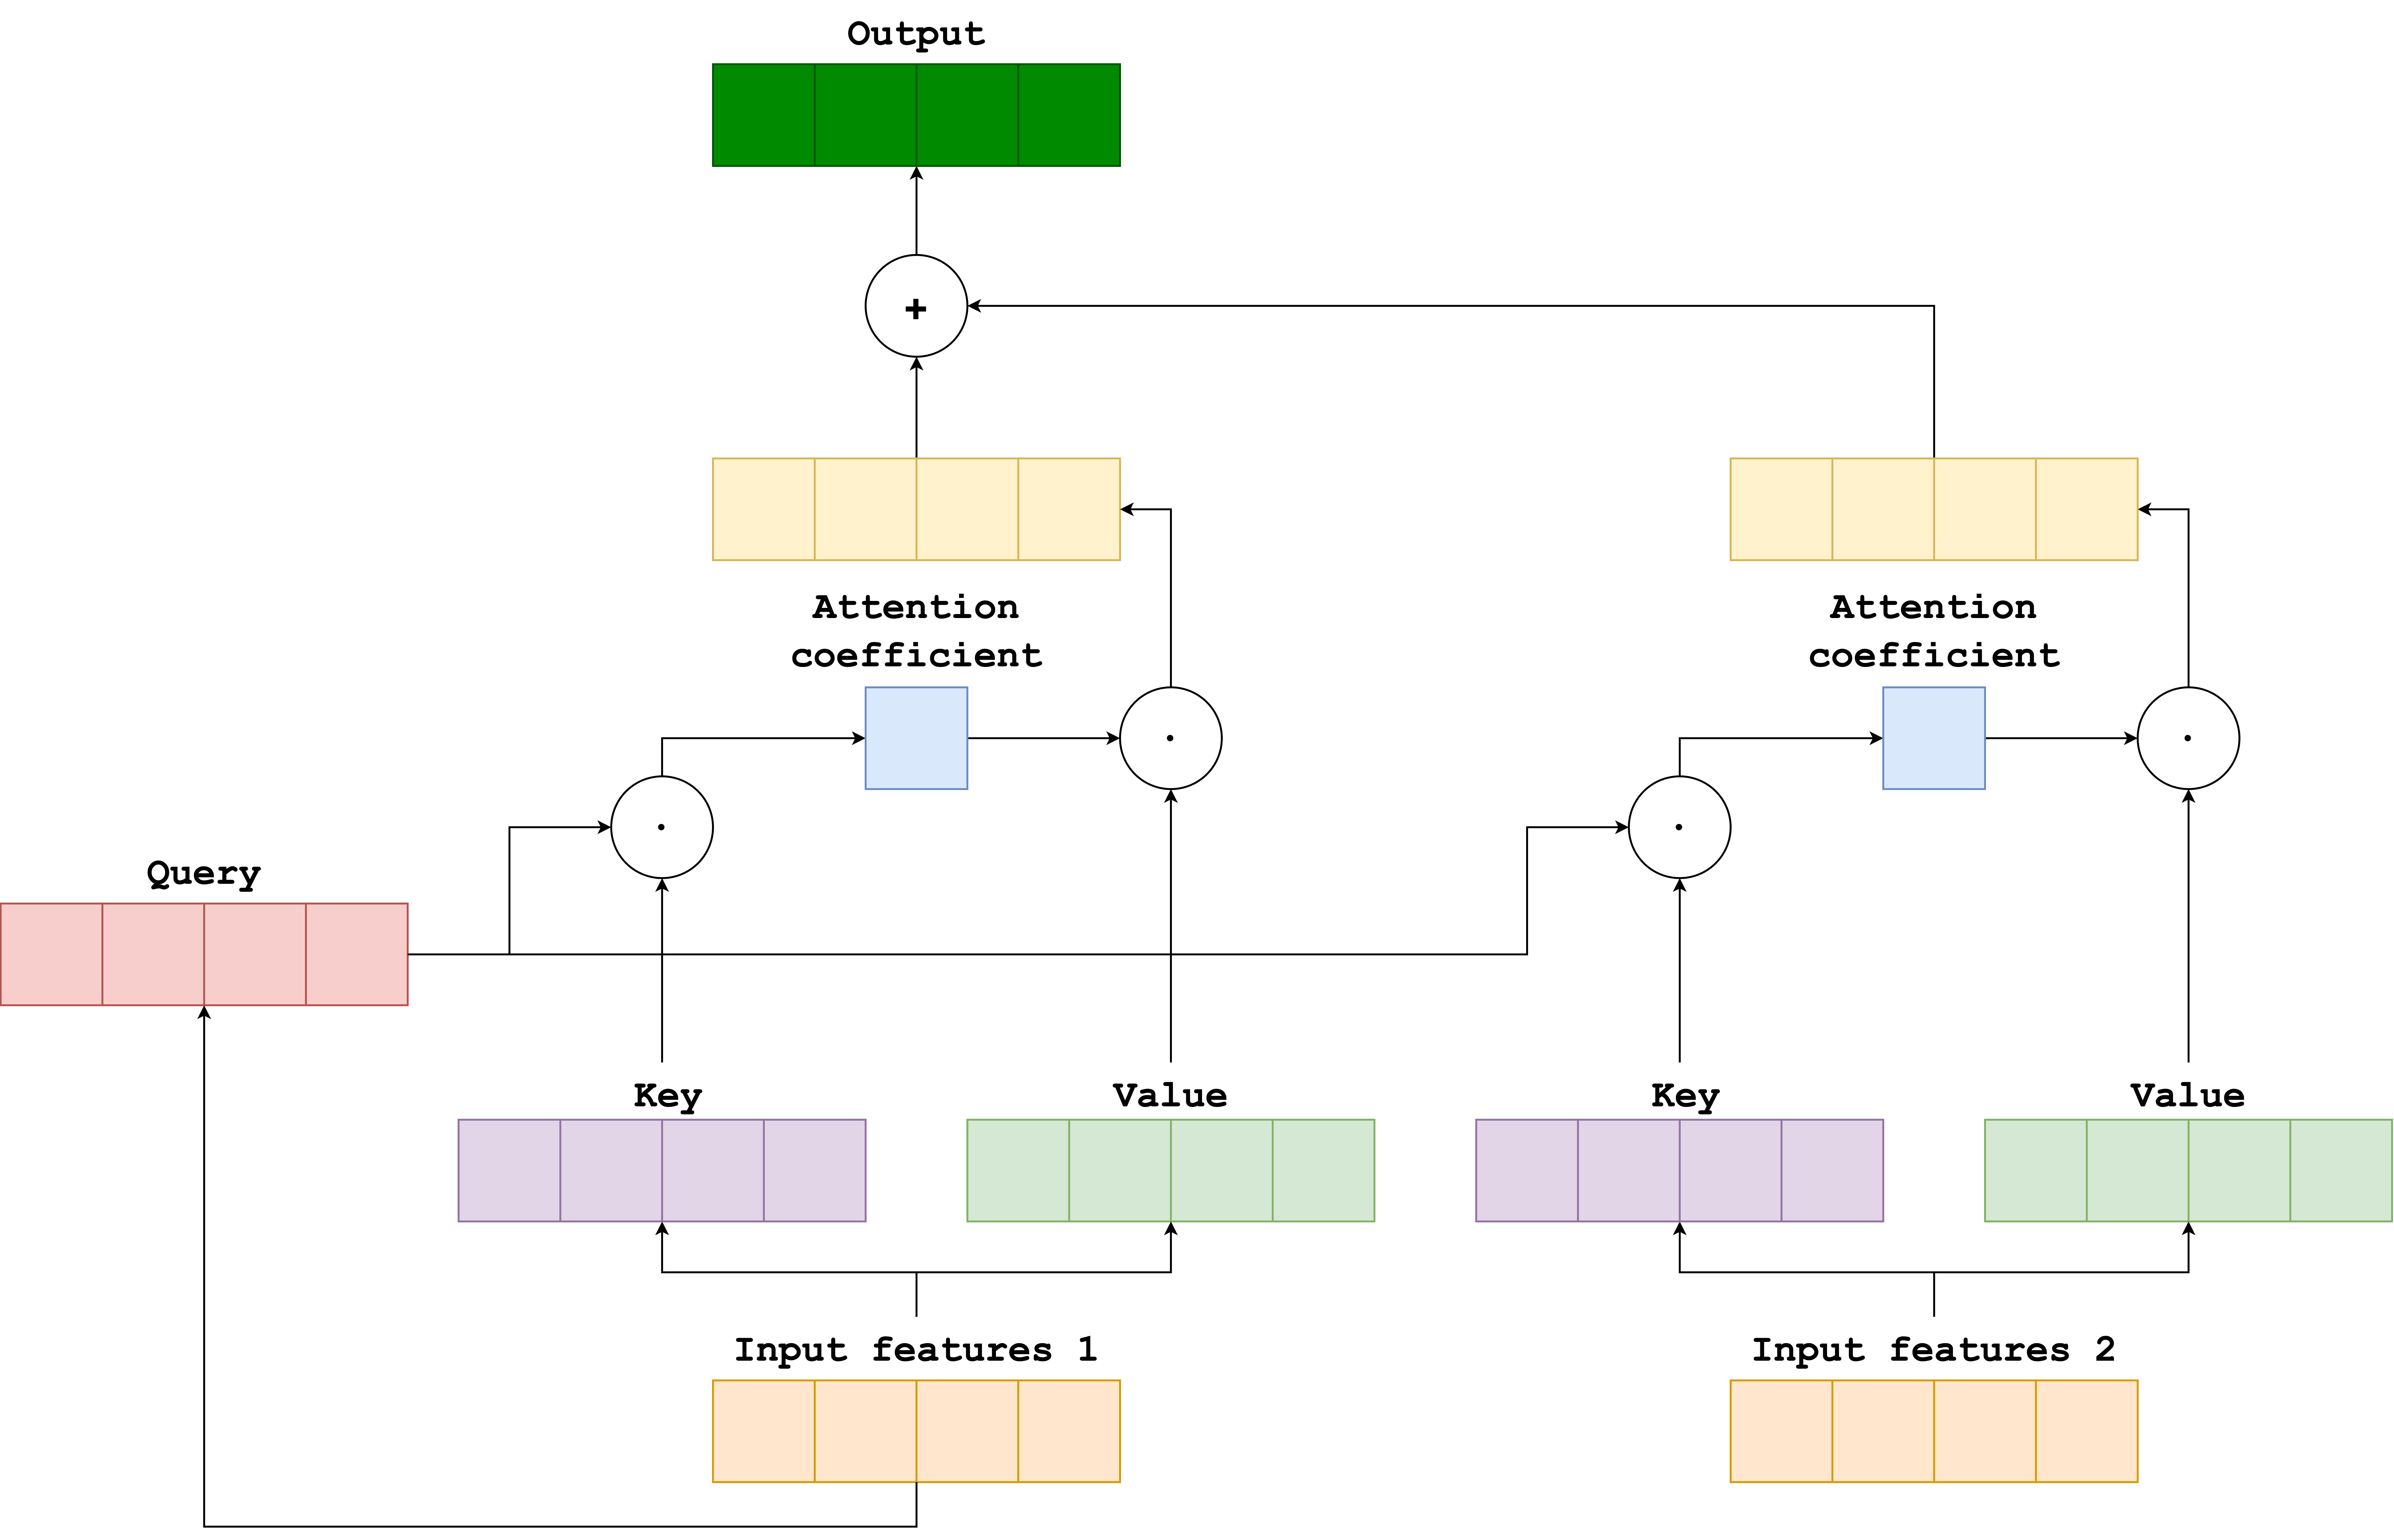
\includegraphics[width=0.8\textwidth]{masters-report/figures/attention-mechanism.png}
    \caption{Overall idea of the self-attention mechanism used in \citet{vaswani2017attention}. Note that the operation that combines the key and the query is highly dependent on the architecture used; for the sake of simplicity, I illustrate the scalar dot product.}
    \label{attention}
\end{figure}

\citet{gat} expanded the attention principle to the realm of GNNs by introducing \text{Graph Attention Networks} (GATs). The attention mechanism proposed by the authors allows the model to focus on different neighbours of a node while aggregating information from its neighbourhood. It assigns attention weights to the neighboring nodes based on their relevance to the target node. The attention weights are learned during the training process and reflect the importance of each neighbour for the target node.

In this work, we are using a version of the GAT network that applies the \textit{self-attention} principle to both scalar and geometric features, allowing the model to learn structural information. \citet{eqgat} propose the \textbf{Equivariant Graph Attention Network} (EQGAT), a model that is equivariant to 3D rotations and translations.

\paragraph{The attention mechanism.} Using a similar notation to the one in Section \ref{the-gvp-math}, for a graph $\mathcal{G} = (\mathcal{V}, \mathcal{E})$, given two nodes $i, j \in \mathcal{V}$ with scalar features $\mathbf{h}_i, \mathbf{h}_j \in \mathbb{R}^{n}$ and edge vector features $\mathbf{e}_{ji}\in \mathbb{R}^n$, we first compute the \textit{query} and \textit{key} vectors by passing the features through two linear layers:
\begin{align}
    \mathbf{q}_i &= \mathbf{W}_q\mathbf{h}_i + \mathbf{b}_q \in \mathbb{R}^n\\
    \mathbf{k}_j &= \mathbf{W}_k\mathbf{h}_j + \mathbf{b}_k \in \mathbb{R}^n
\end{align}
We then take the element-wise product of the key, query and edge features and apply a linear transformation to it to retrieve a vector of attention coefficients $\mathbf{a}_{ji} \in \mathbb{R}^{n + 2\nu}$:
\begin{align}
    \mathbf{\Tilde{a}} &= \mathbf{q}_i \odot \mathbf{k}_j \odot \mathbf{e}_{ji} \\
    \mathbf{a}_{ji} &= \mathbf{W}_a\mathbf{\Tilde{a}}_{ji} = [\Tilde{\mathbf{\alpha}}_{ji}, \mathbf{\beta}_{ji}, \mathbf{\gamma}_{ji}]
\label{attention-coeffs}
\end{align}
The vector $\Tilde{\mathbf{\alpha}}_{ji} \in \mathbb{R}^{n}$ is then used to compute the final attention coefficients for the \textit{scalar features} as follows:
\begin{equation}
    \mathbf{\alpha}_{ji} = \frac{\sigma(\Tilde{\mathbf{\alpha}}_{ji})}{\sum\limits_{j':(j'\rightarrow i)\in\mathcal{E}}\sigma(\Tilde{\mathbf{\alpha}}_{ji})} \in (0, 1)^{n}
\end{equation}
We then compute the \textit{value} tensors for the attention mechanism using weight matrices $\mathbf{W}_{sv}\in\mathbb{R}^{n\times (n+2\nu)}$ and $\mathbf{W}_{vv}\in\mathbb{R}^{n\times n}$:
\begin{align}
    \label{value-tensors} \mathbf{v}_{s, j} &= [\mathbf{v}_{s_0}, \mathbf{y}_{v_0, j}, \mathbf{y}_{v_1, j}] = \mathbf{W}_{sv}\mathbf{h}_j + \mathbf{b}_{sv}  
    \\ \vec{\mathbf{v}}_{v, j} &= \vec{\mathbf{v}}_j\mathbf{W}_{vv}
\end{align}

Finally, we extend the attention mechanism to the vector features. Given that we have initial vector features $\vec{\mathbf{v}}_i, \vec{\mathbf{v}}_j$ for nodes $i$ and $j$, we create vector attention coefficient $\vec{\mathbf{a}}_{v, ji}$ as follows:
\begin{equation}
    \vec{\mathbf{a}}_{v, ji} = \vec{\mathbf{v}}_j \times \vec{\mathbf{v}}_i + \vec{\mathbf{v}}_{v, j}
\end{equation}

\paragraph{Message construction.}
Once we have constructed all necessary features for the attention mechanism, we can compute the incoming messages for the message-passing framework. First, the scalar message from node $j$ to node $i$ is computed as:
\begin{equation}
    \mathbf{m}_{s, ji} = \mathbf{\alpha}_{ji}\odot\mathbf{v}_{s_0, j}
\end{equation}
Next, we compute two types of vector messages from node $j$ to node $i$ using the coefficients computed in Equation \ref{attention-coeffs} and the value tensors computed in Equation \ref{value-tensors}:
\begin{align}
    \mathbf{m}_{v_0, ji} &= \mathbf{\beta}_{ji}\odot \mathbf{y}_{v_0, j}\\
    \mathbf{m}_{v_1, ji} &= \mathbf{\gamma}_{ji}\odot \mathbf{y}_{v_1, j}    
\end{align}
We use these vector messages to construct \textit{equivariant interactions} between nodes $j$ and $i$ by using their relative position $\vec{p}_{ji} = \vec{p}_i - \vec{p}_j$ in 3D space. More formally, we obtain the normalised position $\vec{p}_{e,ij} = \frac{\vec{p}_{ij}}{||\vec{p}_{ij}||_2}$ and combine this with vector message $\mathbf{m}_{v_0,ji}\in\mathbb{R}^n$ through the cross product:
\begin{align}
    \vec{\mathbf{y}}_{0, ji} &= \vec{p}_{e,ij}\otimes\mathbf{m}_{v_0,ji} = \vec{p}_{e,ij}\mathbf{m}_{v_0, ji}^{\top} \in \mathbb{R}^{3\times\nu}
\label{position-cross-product} \\
    \vec{\mathbf{y}}_{1, ji} &= (\mathbf{1}\otimes\mathbf{m}_{v_1, ji})\odot \vec{\mathbf{a}}_{v, ji}\text{, where }\mathbf{1}\in\mathbb{R}^3
\end{align}
\paragraph{Message aggregation.}
The final aggregated message that we form for node $i$ sums the messages received from each of its neighbours on the scalar and vector channels, respectively:
\begin{align}
    \mathbf{m}_{s, i} &= \sum_{j\in\mathcal{N}(i)}\mathbf{m}_{s, ji}\\
    \mathbf{m}_{v, i} &= \sum_{j\in\mathcal{N}(i)}(\vec{\mathbf{y}}_{0, ji} + \vec{\mathbf{y}}_{1, ji}) \\
    \mathbf{m}_i &= (\mathbf{m}_{s, i}, \mathbf{m}_{v, i})
\end{align}

\paragraph{Update.} The last step within a message-passing step is the update. For the update, the authors first sum together the updated state $\mathbf{m}_i$ and the previous state $\mathbf{x}_i = (\mathbf{h}_i, \vec{\mathbf{v}}_i)$:
\begin{equation}
    \mathbf{\Tilde{x}}_i = \mathbf{x}_i + \mathbf{m}_i
\end{equation}
Notice how in this way we combine information about the node's previous state $\mathbf{x}_i\in\mathbb{R}^n\times\mathbb{R}^{3\times\nu}$ with the newly created message $\mathbf{m}_i$. The last step in this layer is to perform a pointwise update using \textit{gated equivariant non-linearities}. The update step is similar to the one in the GVP-GNN architecture and is described in Figure \ref{eqgat}(b). A diagram of the overall EQGAT architecture can be found in Figure \ref{eqgat}. 

% More formally, given the state $\mathbf{\Tilde{x}}_i = (\mathbf{s}_i, \vec{\mathbf{v}}_i)$, we apply two linear transformations $\mathbf{W}_{u_1}$ and $\mathbf{W}_{u_2}$ to the vector features $\vec{\mathbf{v}}_i$:
% \begin{align}
%     \vec{\mathbf{u}}_1 &= \mathbf{W}_{u_1} \cdot \vec{\mathbf{v}}_i \\
%     \vec{\mathbf{u}}_2 &= \mathbf{W}_{u_2} \cdot \vec{\mathbf{v}}_i 
% \end{align}
% We allow information flow from the vector dimension to the scalar dimension by concatenating the norm of $\vec{\mathbf{u}}_1$, namely $\mathbf{n} = ||\vec{\mathbf{u}}_1||_2 \in \mathbb{R}^{\nu}$ to $\mathbf{s}_i$ and passing it through a multilayer perceptron with a SiLU nonlinearity. We obtain three embeddings, $\mathbf{u}_{s_1}, \mathbf{u}_{s_2} \in \mathbb{R}^{n}$ and $\mathbf{u}_v \in \mathbf{R}^\nu$, that we will be using in the final update operation:
% \begin{equation}
%     [\mathbf{u}_{s_1}, \mathbf{u}_{s_2}, \mathbf{u}_v] = \text{MLP}(\text{concat}(\mathbf{s}_i, \mathbf{n}))
% \end{equation}
% We can now obtain the updated scalar and vector features:
% \begin{align}
%     \mathbf{h}_i' &= \mathbf{u}_{s_1} + \mathbf{n}^2 \odot \mathbf{u}_{s_2} \\
%     \mathbf{\vec{v}}_i' &= \mathbf{u}_v \odot \vec{\mathbf{u}}_2
% \end{align}

\begin{figure}
    \centering
    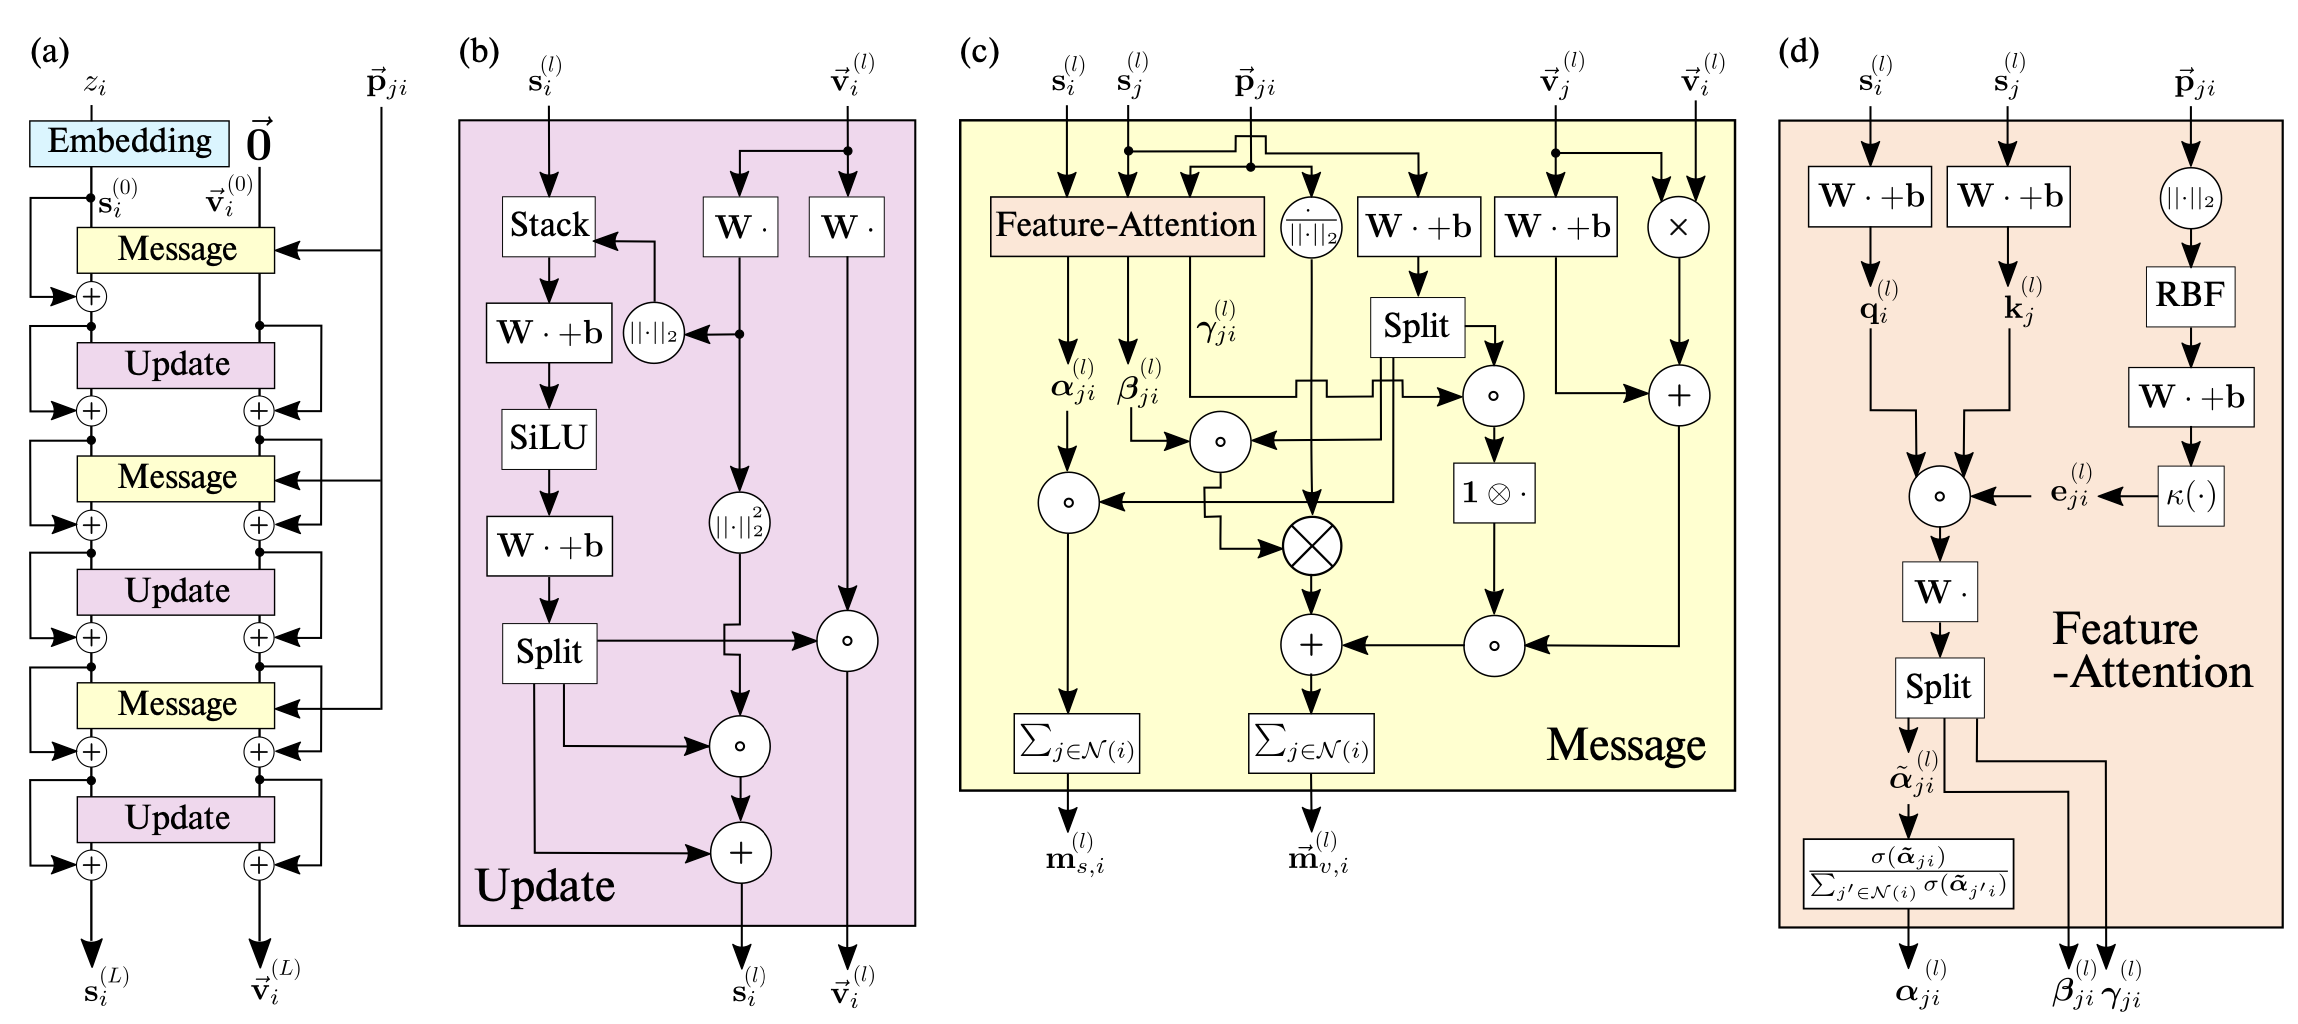
\includegraphics[width=\textwidth]{masters-report/figures/eqgat_diagram.png}
    \caption{(a) The overall message-passing architecture of the EQGAT. (b) The \textit{update} step, allowing information flow from the vector features to the scalar features. (c) The \textit{message construction} step, which creates scalar and vector messages. (d) The \textit{feature-attention} module. Image taken from \cite{eqgat}. }
    \label{eqgat}
\end{figure}

\paragraph{Initial features.}
The initial scalar features used in the model are embeddings created from the atom type of each node, while the initial vector features are set to $\vec{\mathbf{0}}$. Note that after one message-passing layer equivariant vector features are created through the cross-product in Equation \ref{position-cross-product}, which combines the positions of each node with the value tensors created from scalar features. 

Additionally, the edge embedding $\mathbf{e}_{ij}$ encodes the distance between node $i$ and node $j$. We embed the interatomic distance $d_{ij} = ||p_{ij}||_2 \in \mathbb{R}$ using the Bessel radial basis function (RBF), formally defined as:
\begin{equation}
    \text{RBF}_k(d_{ji}) = \sqrt{\frac{2}{c}\frac{\sin(\frac{k\pi}{c}d_{ji})}{d_{ji}}}
\end{equation}
for distance cutoff $c$ and $k = 1, \dots, K$. We concatenate $\text{RBF}_k(d_{ji})$ for all $k = 1,\dots,K$ to obtain an initial edge features $\mathbf{e}^{\text{RBF}}_{ij}$. We pass these through a trainable linear layer and obtain:
\begin{equation}
    \Tilde{\mathbf{e}}_{ji} = \mathbf{W}_e\mathbf{e}^{\text{RBF}}_{ij} + \mathbf{b}_e
\end{equation}
To obtain the final edge embedding, we combine $\Tilde{\mathbf{e}}_{ji}$ with a cosine-cutoff function. The final edge embedding becomes:
\begin{equation}
    \mathbf{e}_{ji} = \frac{1}{2}\Big(\cos (\frac{\pi d_{ji}}{c}) + 1\Big)\cdot \mathbbm{1}[d_{ji}\leq c]\cdot \Tilde{\mathbf{e}}_{ji}
\end{equation}

\subsection{Training hyperparameters}
\label{training-details}
I train two equivariant GNN models on the RES task using the ATOM3D RES dataset \cite{atom-3d}. Both models are trained using one NVIDIA A100 GPU provided by the University's HPC Cluster.  Table \ref{hyperparameters} summarises the hyperparameter configuration of both of my models. Since \citet{eqgat2} do not report the configuration used for training the EQGAT model on the RES task, I instead use the one proposed in the GVP paper for both models. Due to computational constraints, I was unable to perform hyperparameter validation, but I achieve a new state-of-the-art performance on the GVP model, as discussed in Section \ref{sec:res-task}.

\begin{table}[!h]
\centering
\caption{Model architectures and training configuration.}
\vskip 0.15in
\label{hyperparameters}
\begin{tabular}{@{}llll@{}}
\toprule
Hyperparameter                  & \multicolumn{1}{l|}{Value}     & Hyperparameter     & Value     \\ \midrule
Message-passing layers          & \multicolumn{1}{l|}{5}         & Learning rate      & $10^{-4}$ \\
Node features (scalar, vector)  & \multicolumn{1}{l|}{(100, 16)} & Patience scheduler & 10        \\
RBFs                            & \multicolumn{1}{l|}{32}        & Decay rate         & 0.75      \\
RBF cutoff                      & \multicolumn{1}{l|}{4.5 \AA}   & Dropout            & 0.1       \\
EQGAT RBF function              & \multicolumn{1}{l|}{Bessel}    & Batch size         & 64        \\
GVP RBF function                & \multicolumn{1}{l|}{Gaussian}  & Epochs             & 40        \\ \midrule
EQAT total learnable parameters & 469 K                          &                    &           \\
GVP total learnable parameters  & 386 K                          &                    &           \\ \bottomrule
\end{tabular}
\end{table}

\section{Mutation generation}
\label{sec:mutation-generation}
This section describes the strategy used to generate mutations using the two trained GNN models described in Sections \ref{the-gvp-math} and \ref{eqgat-math}. These models are trained to predict the most likely amino acid given a local atomic environment. Based on these capabilities, I repurpose them to the task of mutation generation by masking out each amino acid in a structure \textit{in turn} and passing the masked structure through the model. I then use the scores $l \in \mathbb{R}^{20}$ defined in Equation \ref{logit-scores} to rank the most likely amino acids for each position. Figure \ref{mutation-generation} illustrates this approach visually. 

\begin{figure}[!h]
    \centering
    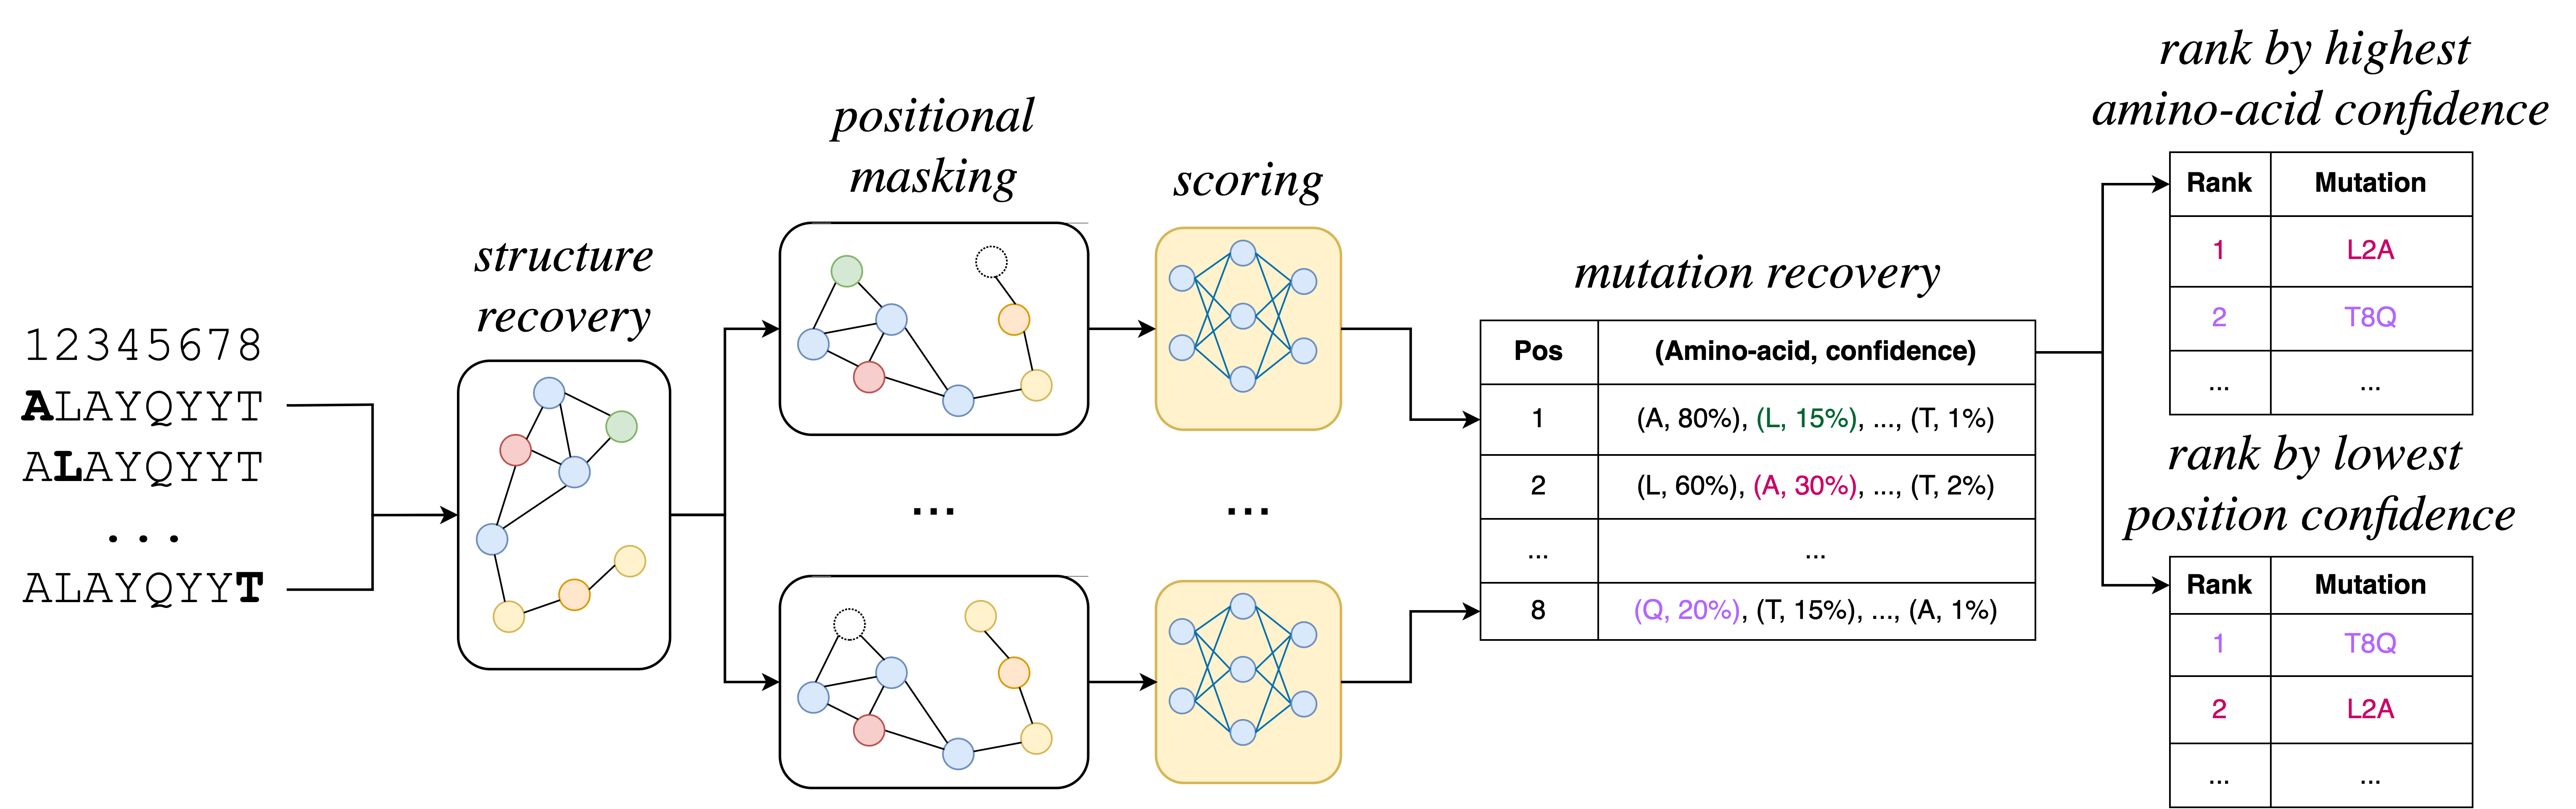
\includegraphics[width=\textwidth]{masters-report/figures/mutation_generation_final.png}
    \caption{Pipeline of phase 2.}
    \label{mutation-generation}
\end{figure}


\subsection{Structure recovery}
\label{sec:structure-recovery}

The ProteinGym substitutions dataset \cite{tranception} contains 87 wildtype sequences. For each of these sequences, a number of experimentally tested mutations are scored according to their \textit{fitness}. While the dataset also includes the fitness of sequences that have been mutated at multiple positions, the scope of this project is limited to \textit{single-point} mutations. 

\paragraph{Monomers and oligomers.} 
As explained in Section \ref{sec:biological-background}, some proteins are part of assemblies. 
When inducing a mutation into a protein that is part of a protein assembly, it must be replicated across all identical chains in the complex. Due to this constraint, I reduce the scope of this project to only deal with sequences whose structures are either \textit{monomers} or \textit{homo-oligomers}. 

The ProteinGym dataset does not provide a mapping between sequences and structures, so the first part of the pipeline illustrated in Figure \ref{mutation-generation} involves the recovery of structures from the Protein Data Bank \cite{rcsb_pdb}. I query the PDB through their programmatic API\footnote{\url{https://search.rcsb.org/index.html\#search-api}} for the biological assembly associated with a sequence. When multiple assemblies are available for the same sequence, I choose the first one returned by the query. 

These assemblies are determined experimentally using X–ray crystallography.\footnote{X-ray crystallography is a method that involves exposing a crystallised sample of a molecule to X-rays in order to determine the positions of individual atoms.} Some experimental assemblies have two challenges. Firstly, the molecule may be bound to a ligand,\footnote{A ligand is usually a smaller molecule that is attached to the main protein and helps it stabilise.} so X-ray crystallography will reveal both the positions of the atoms in the main protein and the atoms in the ligand. To solve this, I apply a post-processing step that cleans the assembly of any undesired ligands or water molecules; the cleaning code is inspired by an approach taken in the AlphaFold \cite{alphafold} codebase.

Secondly, some proteins contain inherently mobile chains that cannot be crystallised. When this is the case, the biological assembly will have an incomplete structure, so I discard the experimental structure and instead use the AlphaFold structural prediction.

\paragraph{AlphaFold structures.} AlphaFold can only predict the structure of monomers. This means that it cannot be easily used to build up hetero-oligomers, and for homo-oligomeric assemblies it will only predict the monomer from which the complex is formed, as exemplified in Figure \ref{alpha-fold-monomer}. The major drawback of using a monomer instead of the entire biological assembly to generate mutations is that amino acids lying on the outskirts of a molecule may be wrongly flagged as viable for mutations, when in reality they should bind to other copies of themselves. A more thorough analysis of the impact of using AlphaFold structures instead of biological assemblies is discussed in Chapter \ref{results}, where an ablation study compares the performance difference when using predicted monomers instead of the full biological assembly.

\begin{figure}[!h]
\centering
    \subfigure[The 6EZM molecule, commonly known as Baker's Yeast. It is formed of 24 copies of the same monomer.]{
        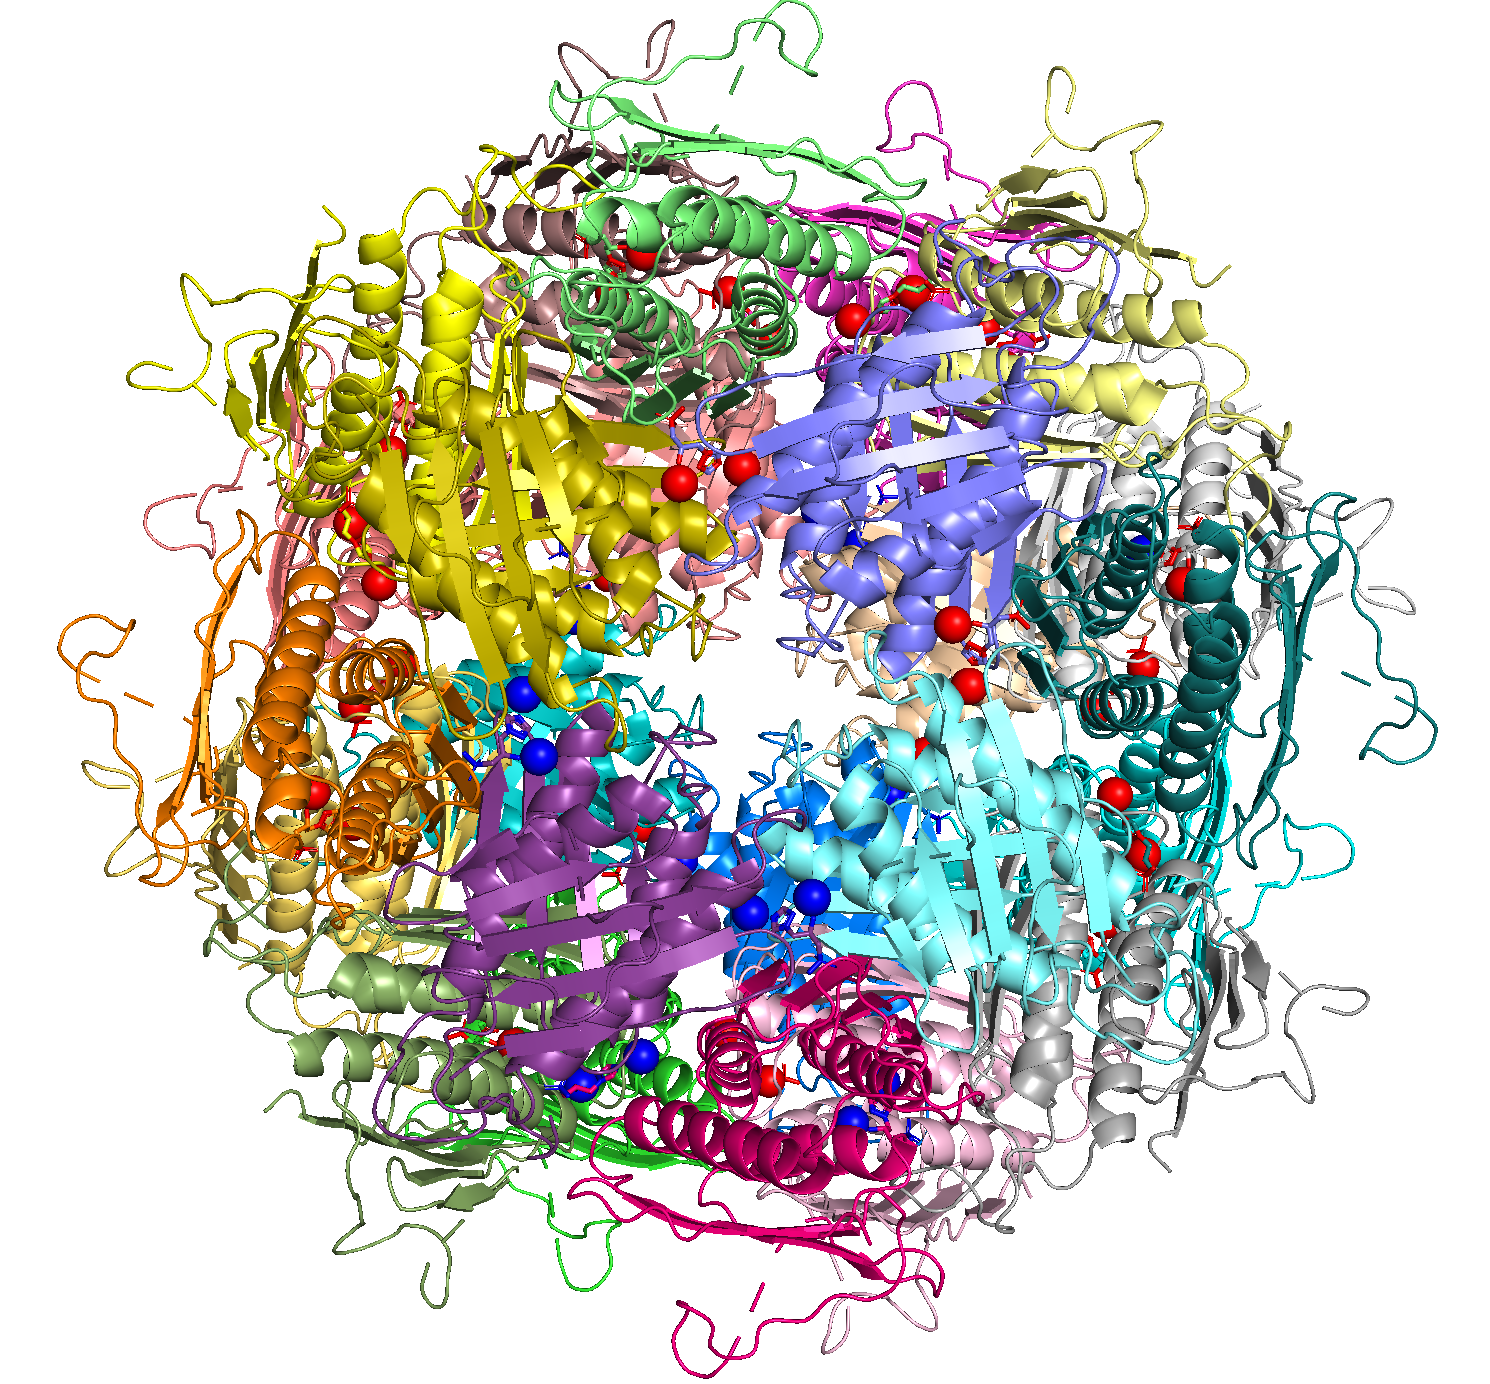
\includegraphics[scale=0.20]{masters-report/figures/6ezm-yeast.png}
        \label{monomer}
    }
    \hspace{0.2in}
    \subfigure[The monomer predicted by AlphaFold for the 6EZM molecule.]{
        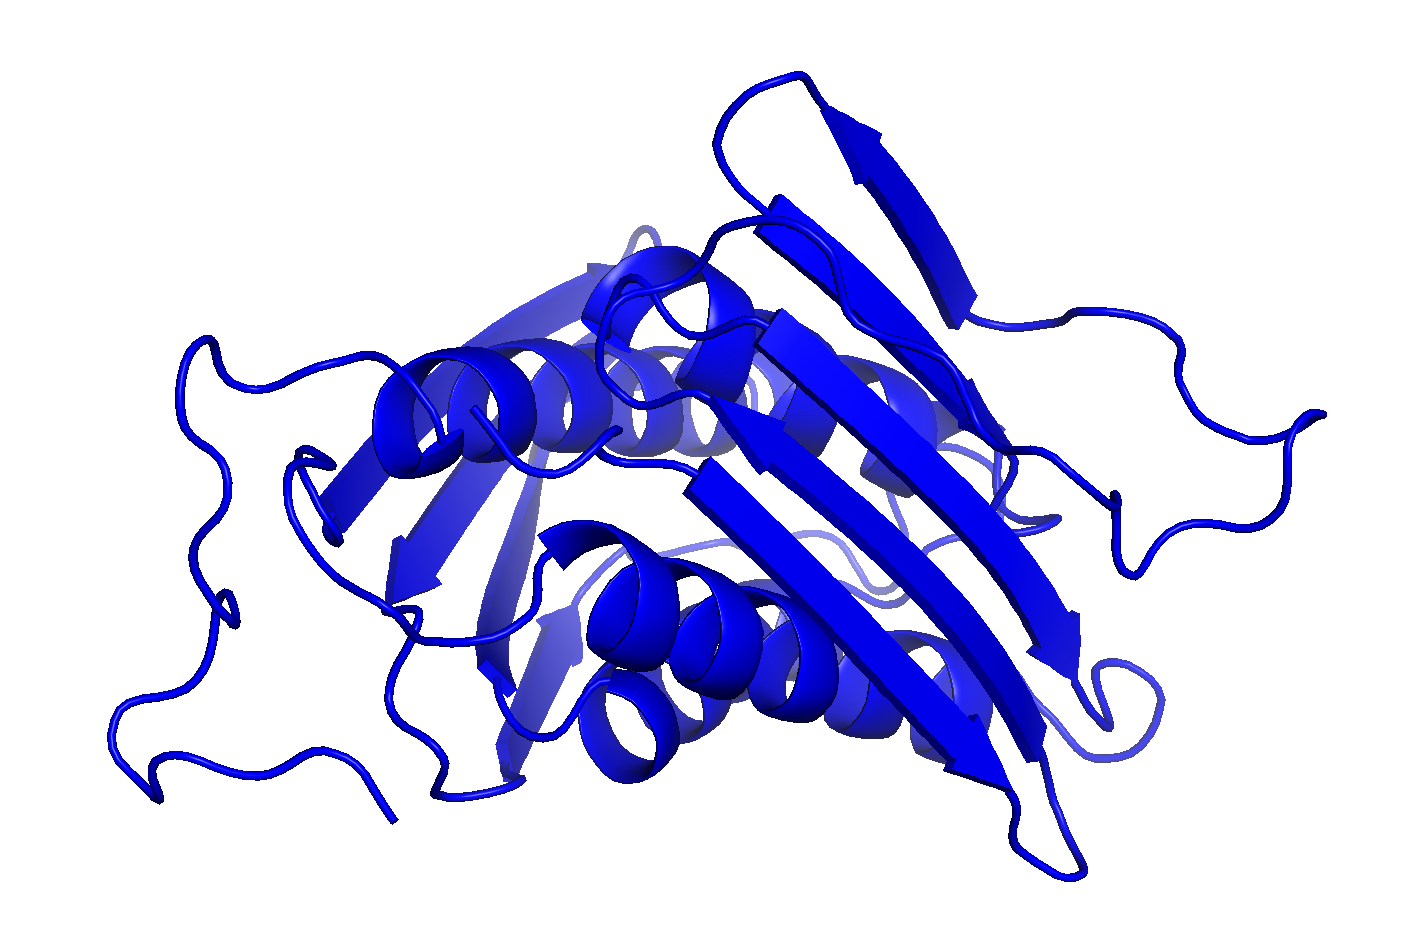
\includegraphics[scale=0.20]{masters-report/figures/alpha-fold-pred.png}
    }
    \caption{Example of (a) a mono 24-mer and  (b) the AlphaFold prediction for the sequence of the mono 24-mer.}
    \label{alpha-fold-monomer}
\end{figure}

The overall structure processing pipeline is presented in Figure \ref{filtering-steps}, which highlights all the points during the post-processing of structures where a design decision is made. 
\begin{figure}[!h]
    \centering
    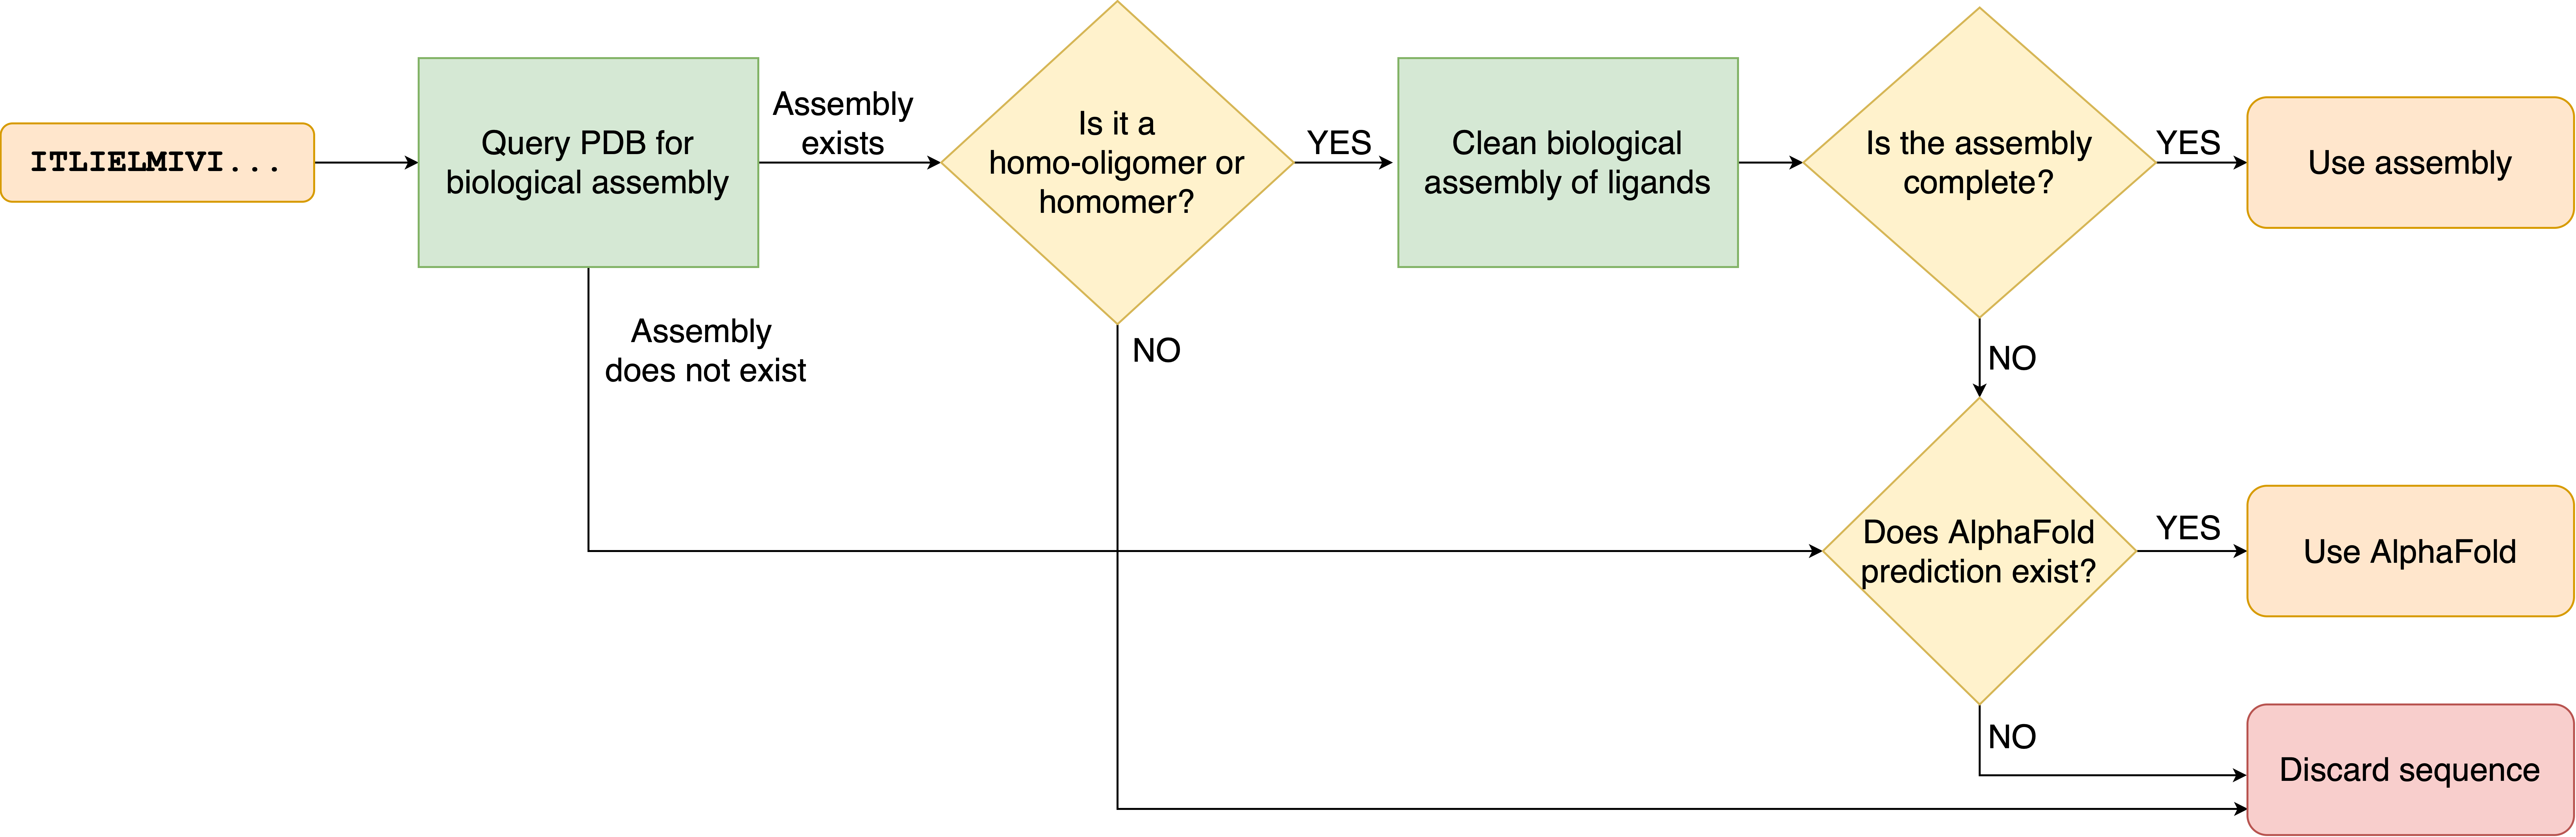
\includegraphics[width=\textwidth]{masters-report/figures/data-process.png}
    \caption{The structure processing pipeline.}
    \label{filtering-steps}
\end{figure}

\subsection{Positional masking}
\label{positional-masking}
The main idea behind the mutation generation strategy is that for every sequence for which I have obtained a clean structure according to the filtering pipeline presented in Figure \ref{filtering-steps} I follow the steps below to determine all possible single-point amino acid mutations in the sequence:
\begin{enumerate}
    \item Firstly, I mask the amino acid residue present at a target position in the structure; 
    \item Secondly, I pass the masked structure through the GNN model; 
    \item Thirdly, I recover the score corresponding to the probability of each of the 20 naturally-occurring amino acids to be in the masked position. 
\end{enumerate}
I repeat this process for all positions in the sequence. 
Intuitively, a higher probability (i.e., model confidence) for a \textit{residue} indicates that the model believes it would be a good match for that position; conversely, an overall lower confidence at a target \textit{position} indicates the position is amenable to mutations.

\subsection{Mutation ranking}
Once I have the scores associated with each of amino acid mutation for every position in a sequence, I propose two strategies for ranking these mutations: global and positional. Formally, given a wildtype sequence $x_1x_2\dots x_n$ of length $n$ with $x_i \in \mathcal{A} = \{1,2,\dots,20\}$ representing the index of amino acid $i$, associated to a atomic graph $\mathcal{G} = (\mathcal{V}, \mathcal{E})$, the process described in \ref{positional-masking} builds a scoring function of the positions  $S:\{1,2,\dots,n\}\times\mathcal{A}\rightarrow \mathbb{R}$ that I define by extending the formalism in Equation \ref{full-formalism}:
\begin{equation}
    S(i, a) = [f_{\gamma}^{g(i)}(\mathbf{H}, \mathbf{E})]_a
\label{scoring-function}
\end{equation}
Where $g:\{1,2,\dots,n\}\rightarrow\{1,2,\dots,|\mathcal{V}|\}$ is a mapping function from positions to the index of the node representing the central $\text{C}_{\alpha}$ of the residue present at said position. 

Equation \ref{scoring-function} essentially represents the score of amino acid $a$ for target position $i$, associated with node $g(i)$ in the atomic graph. Note that the true amino acid at the same position is denoted by $x_i$. 
We are now ready to formally define the two ranking strategies. 

\paragraph{Global ranking.} The first approach to ranking the scores of our mutations is to sort them in descending order of their scores, regardless of the position they occupy. If we denote the single-point mutation to amino acid $a$ at position $i$ by $\mathbf{m}_{i}^a$, then $\forall i,j\text{ and }\forall a,b\in \mathcal{A} \text{ s.t. } a \neq x_i \text{ and } b \neq x_j$, we say that:
\begin{equation}
    \mathbf{m}_{i}^a\text{ is better than }\mathbf{m}_{j}^b \iff S(i, a) > S(j, b)
\label{global-ranking}
\end{equation}

\paragraph{Positional ranking.} The second approach follows when I prioritise the positions I want to mutate instead of the amino acids I mutate to. Instead of quantifying mutations by their global score compared to all other mutations, I rank mutations by the confidence of the model in predicting the wildtype residue at each position. Intuitively, if the model confidence in the wildtype residue $x_i$ at position $i$ is low, this is an indication that the position itself may be prone accept mutations. Formally, this can be quantified as:
\begin{equation}
\begin{aligned}
&\mathbf{m}_{i}^a\text{ is better than }\mathbf{m}_{j}^b \\ 
\iff &\Big(S(i, x_i) < S(j, x_j)\Big) \lor \Big(S(i, x_i) = S(j, x_j) \land S(i, a) > S(j, b)\Big)
\end{aligned}
\label{positional-ranking}
\end{equation}
Equation \ref{positional-ranking} ranks mutations first by their positions; that is, the less confident the model is in a wildtype residue at a certain position, the higher any mutation on that position will rank. In the case of ties (when comparing mutations to different amino acids at the same position), I compare the actual mutation score. I then keep only \textit{the top 3} proposed mutations for each position. 

\section{Protein fitness prediction}
\label{protein-fitness-prediction}
As a second extension to the original scope of the project, I propose a straightforward fitness prediction model that can learn from an already existing dataset of single-point mutations to predict the fitness of a sequences. Following an approach similar to the one used for mutation generation in Section \ref{sec:mutation-generation}, I obtain the scores of all single-point amino acid mutations for every position in every wildtype sequence part of the ProteinGym substitutions dataset \cite{tranception}. I use these scores to augment a baseline regression model to perform protein fitness prediction.

% \begin{figure}
%     \centering
%     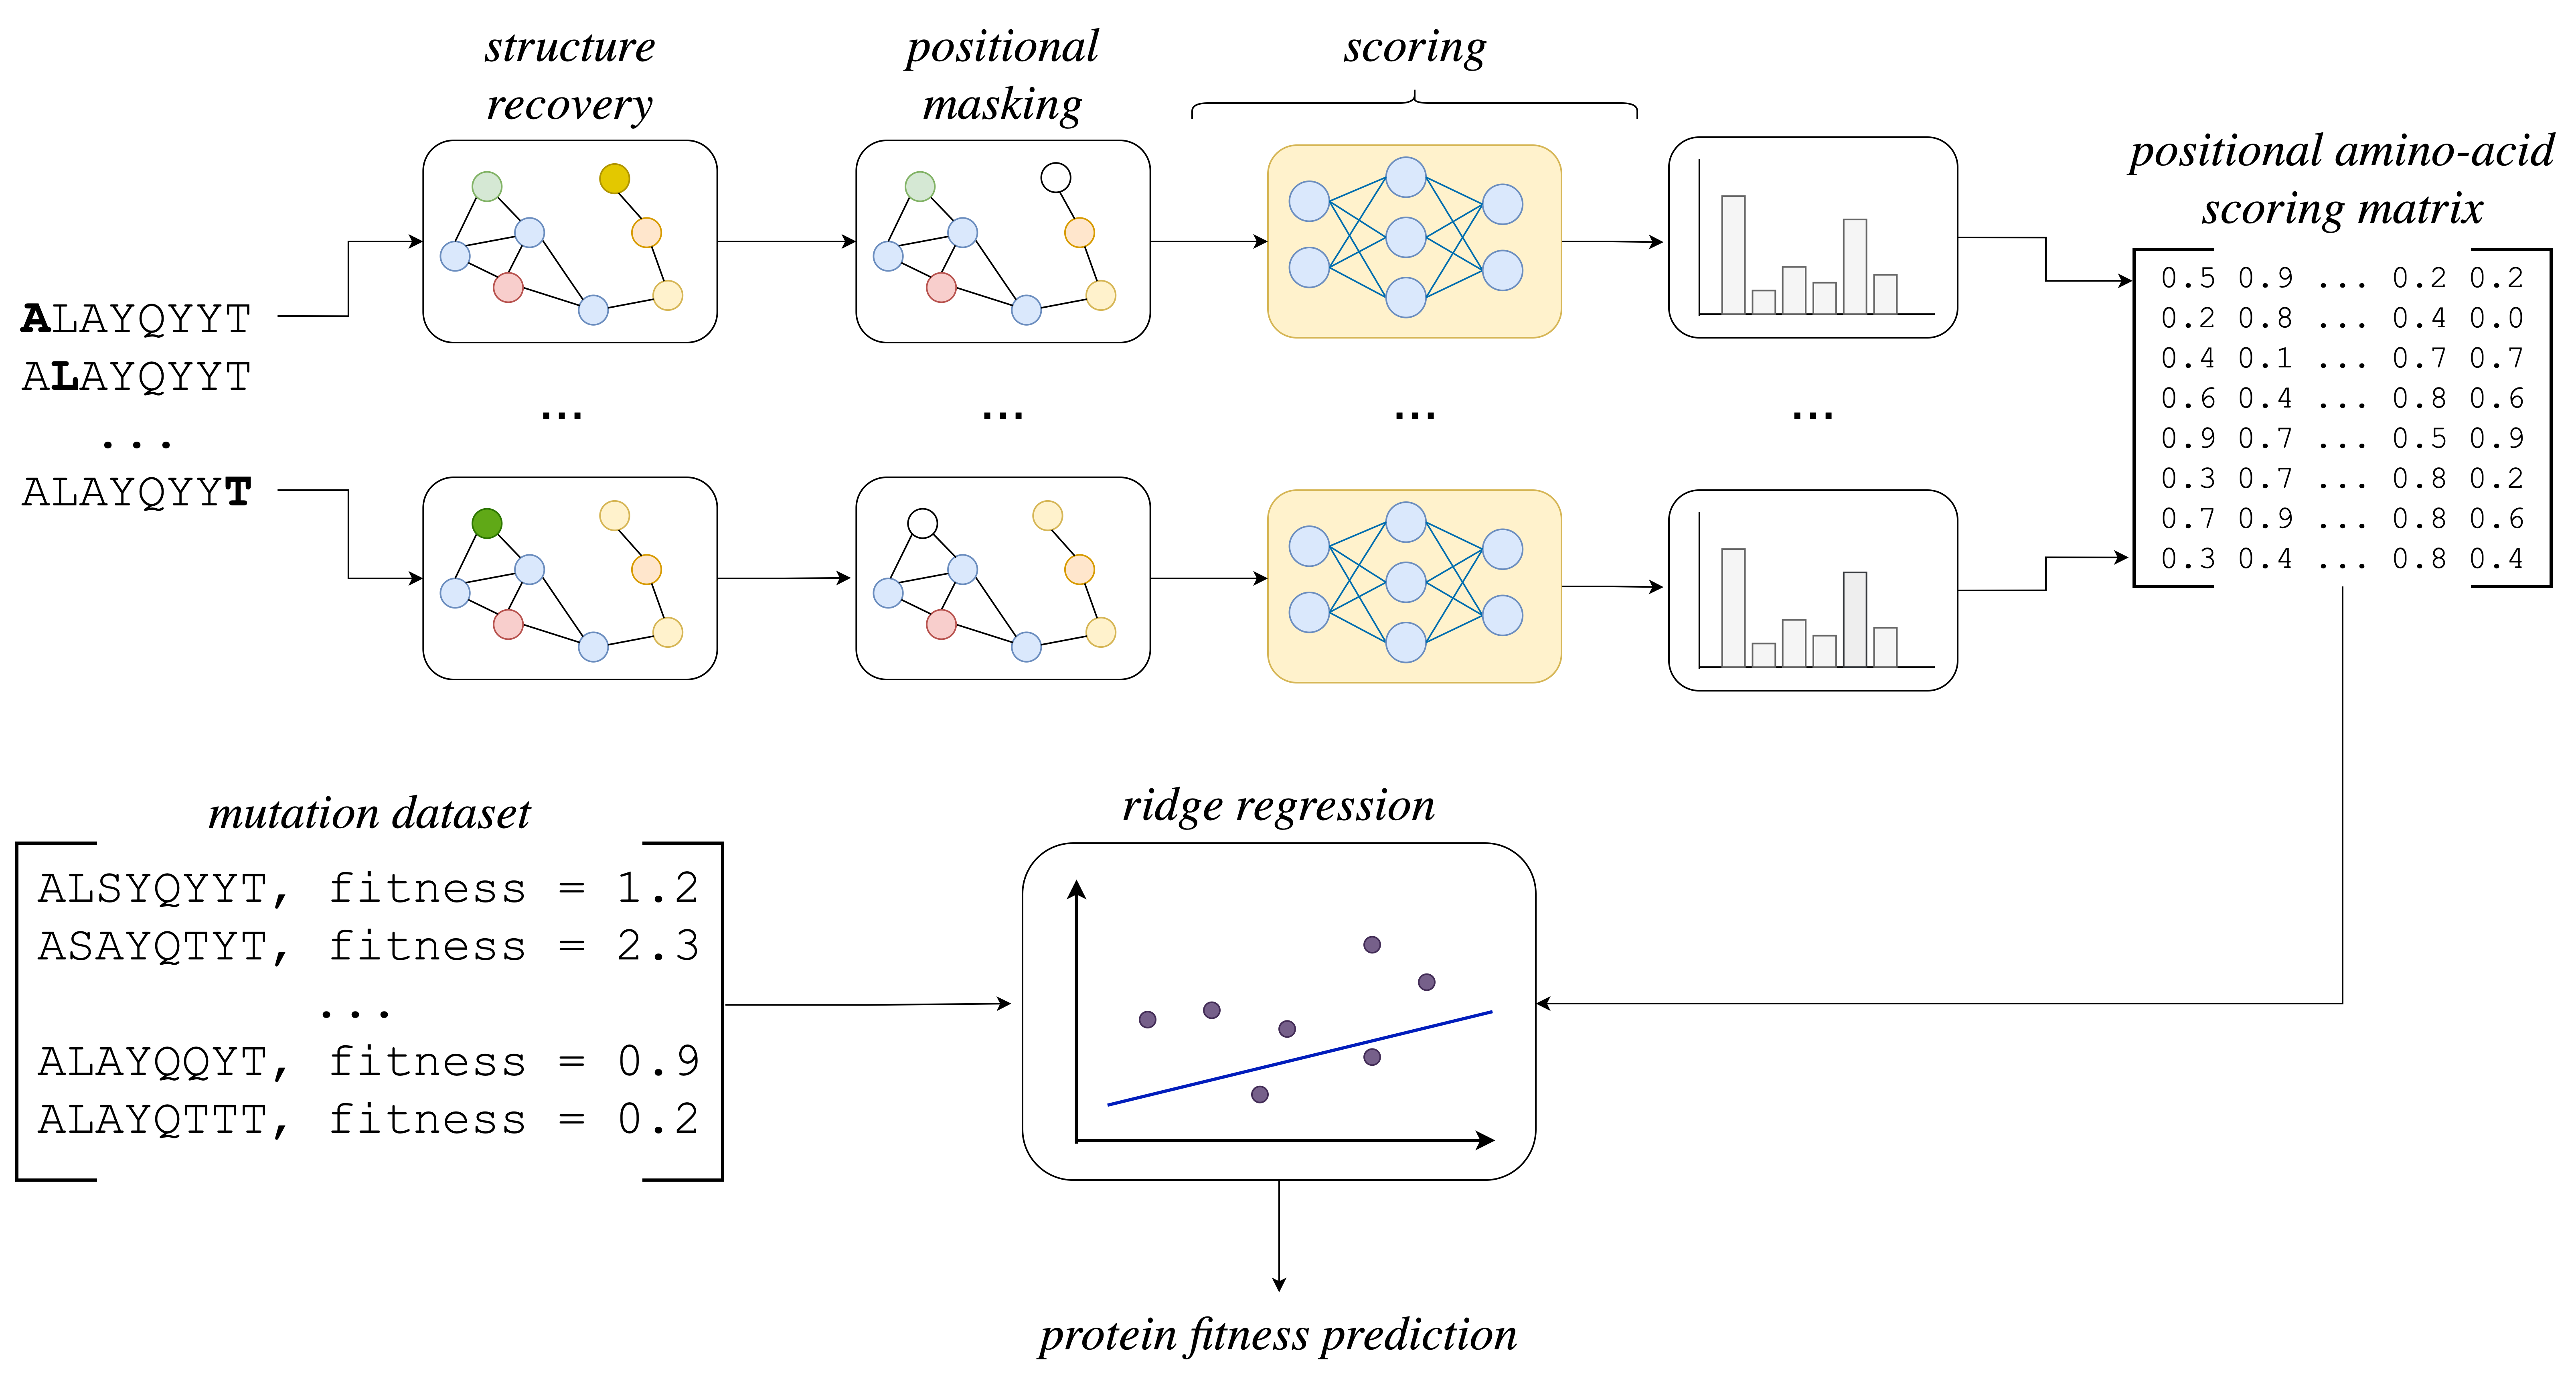
\includegraphics[width=\textwidth]{masters-report/figures/protein_fitness_prediction.png}
%     \caption{Pipeline of phase 3.}
%     \label{fitness-prediction}
% \end{figure}

\subsection{Baseline model} 
I start off with a simple ridge regression model that uses a similar approach to the one proposed by \citet{chloe-hsu}. Formally, for a mutated sequence $s_i = a_1a_2\dots a_n$, we consider its features for the regression to be:
\begin{equation}
    \mathbf{x}_i = [~\text{embed}(a_1) ~||~ \text{embed}(a_2) ~||~ \dots ~||~\text{embed}(a_n)~] ~\in~\mathbb{R}^{n \times d} 
\label{baseline-regression}
\end{equation}
wherd $d\in\mathbb{N}$ is the dimension of the encoding function $\text{embed}:\mathcal{A}\rightarrow \mathbb{R}^d$. The value to predict, $y_i$, represents the fitness of the sequence.

I evaluate two types of encodings in this project:
\begin{enumerate}
    \item The \textbf{one-hot} encoding;
    \item The \textbf{AAIndex} embeddings. The AAIndex database \cite{aa-index} is a database of numeric indicators that represent a wide range of physicochemical and biochemical characteristics of amino acids. I create embeddings from these indices by parsing all known characteristics and performing principle component analysis on them to generate 19-dimensional feature vectors. 
\end{enumerate}

\subsection{Augmented models} 
I augment these simple regression models by adding the score of the single-point mutation present in the sequence $s_i$ to the feature vector $\mathbf{x}_i$. Formally, if sequence $s_i = a_1a_2\dots a_n$ has single-point mutation $\mathbf{m}_i^a$, then the feature vector becomes:
\begin{equation}
    \mathbf{x}_i' = [~\text{embed}(a_1) ~||~ \text{embed}(a_2) ~||~ \dots ~||~ \text{embed}(a_n) ~||~ {\color{blue} S(i, a)}~] ~\in~\mathbb{R}^{n\times d + 1}
\label{augmented-regression}
\end{equation}
Where $S(i, a)$ is the same scoring function as in Equation \ref{scoring-function}. Note that I regularise $S(i,a)$  differently from the rest of the regression features, since the value scale of the score is different from the value scale of the embeddings. This way of creating feature vectors takes into consideration only single-point mutations, hence I add a single new scalar to the feature vector $\mathbf{x}_i$. 
% When dealing with the wildtype sequence, I concatenate either $1$ or $0$ to the original feature vector $\mathbf{x}_i$, depending on the dataset.

% The regression models defined in Equations \ref{baseline-regression} and \ref{augmented-regression} are trained on each wildtype sequence from the ProteinGym dataset separately. These models provide a quick and easy way of predicting the fitness of new mutations given a number of already existing datapoints, hence performing well in a low-data regime. 
\section{Implementation details}

\subsection{Libraries}
The entire implementation of this project was written in the Python programming language.\footnote{\url{https://www.python.org}} I utilised the PyTorch \cite{paszke2019pytorch} and PyTorch Geometric \cite{pyg} frameworks for deep learning components and graph neural network modules. Training was done using PyTorch Lightning,\footnote{\url{https://lightning.ai/docs/pytorch/stable/}} a lightweight wrapper for PyTorch that abstracts away boilerplate code for ML training. I used WandB\footnote{\url{https://wandb.ai/site/papers}} to monitor training runs and log validation metrics. To train the ridge regression models I made use of the \texttt{scikit-learn} Python library.\footnote{\url{https://scikit-learn.org/stable/}}


For processing biological data, I used the following Python libraries: \texttt{biotite}, \texttt{biopandas}, \texttt{biopython}, and \texttt{atom3d}. The former two were used to read and process \texttt{.pdb} files (the format in which protein structures are kept in the Protein Data Bank \cite{rcsb_pdb}), while the latter two were used for miscellaneous biological constants. All protein visualisations presented in this report are generated with PyMol \cite{pymol}.
\subsection{Starting point}
The starting point of this project made use of code from the following three open-source repositories:
\begin{itemize}
    \item \texttt{drorlab/gvp-pytorch}\footnote{\url{https://github.com/drorlab/gvp-pytorch}}: this repository contains the official implementation of the GVP \cite{gvp1, gvp2} module. My supervisor provided an optimised version of this architecture that I could use for faster training on the RES task. I adapted my supervisor's code to fit into my Pytorch Lightning training framework. 
    \item \texttt{Bayer-Group/eqgat}\footnote{\url{https://github.com/Bayer-Group/eqgat}}: this repository contains the official implementation of the EQGAT \cite{eqgat, eqgat2} architecture. I adapted this code to fit into my Pytorch Lightning training framework. 
    \item \texttt{deepmind/alphafold}\footnote{\url{https://github.com/deepmind/alphafold/blob/a3941673e90b8d1d75c60b16a4b3707ebf7ba527/alphafold/relax/cleanup.py}}: this repository contains the official implementation of the AlphaFold \cite{alphafold} model. From here I adapted code to clean experimental protein structures. 
\end{itemize}
For the evaluation against all sequence-based models, I used results available in the \texttt{OATML-Markslab/Tranception} repository.\footnote{\url{https://github.com/OATML-Markslab/Tranception}}